%&tex

\documentclass[14pt]{ffslides}

\ffpage{40}{1.7777}

\usepackage{helvet}
\usepackage[english]{babel}
\usepackage[T1]{fontenc}
\usepackage{wrapfig}
\usepackage{csquotes}
\usepackage{mathtools}
\usepackage{amsfonts}
\usepackage{amsthm}
\usepackage{amssymb}
\usepackage{thmtools,thm-restate}
\usepackage{multicol}
\usepackage{hyperref}
\usepackage{graphicx}
\usepackage{pifont}
\usepackage[singlelinecheck=false]{caption}
\usepackage{algorithm}
\usepackage[noend]{algpseudocode}
\usepackage{subcaption}
\usepackage{booktabs}
\usepackage{textcomp}
\usepackage{xcolor,colortbl}
\usepackage{enumitem}
\usepackage{multirow}
\usepackage{multicol}
\usepackage{pgfplots}
\usepackage{natbib}
\usepackage{bibentry}
\usepackage{bm}
\usepackage{wasysym}
\usepackage{tikz}
\usetikzlibrary{shapes,arrows,positioning,fit,circuits.logic.US}
\pgfplotsset{compat=1.17}

\bibliographystyle{plainnat}

\definecolor{boxgray}{HTML}{808080}
\definecolor{boxdgray}{HTML}{545454}
\definecolor{boxnteal}{HTML}{467085}
\definecolor{boxdgreen}{HTML}{335C33}
\definecolor{boxbrown}{HTML}{4C331A}
\definecolor{boxkpgreen}{HTML}{3beb7e}

\definecolor{boxblue}{HTML}{3275a8}
\definecolor{boxlblue}{HTML}{AFDCFF}
\definecolor{boxorange}{HTML}{ce654f}
\definecolor{boxlorange}{HTML}{cc7d6d}
\definecolor{boxllorange}{HTML}{edaea1}
\definecolor{boxpurple}{HTML}{271F36}
\definecolor{boxred}{HTML}{B44650}
\definecolor{boxgreen}{HTML}{54774B}
\definecolor{boxlgreen}{HTML}{9CD08F}
\definecolor{boxteal}{HTML}{568777}
\definecolor{boxlteal}{HTML}{88C7B2}
\definecolor{boxgold}{HTML}{EFA906}
\definecolor{boxdyellow}{HTML}{F9CB40}
\definecolor{boxgoldenrod}{HTML}{818a34}
\definecolor{boxpink}{HTML}{b522a4}
\definecolor{boxwheat}{HTML}{e1ca96}
\definecolor{boxolive}{HTML}{bbbe64}
\definecolor{boxmunsel}{HTML}{04a777}

\definecolor{pviolet}{HTML}{8332AC}
\definecolor{psandy}{HTML}{6C441E}
\definecolor{pdgreen}{HTML}{219E31}
\definecolor{pbrickred}{HTML}{D1495B}
\definecolor{pyellow}{HTML}{FFE066}

\usepackage{pifont}

\newcommand{\cmark}{\color{boxgreen}\ding{51}}%
\newcommand{\xmark}{\color{boxred}\ding{55}}%
\newcommand{\omark}{{\color{boxblue!40!black}\large$\bm{\bigcirc}$}}%

\newlist{checks}{itemize}{2}
\setlist[checks]{label=$\square$,align=left,labelindent=*}

\newcommand{\bigo}{\mathcal{O}}
\newcommand{\set}[1]{\mathbf{#1}}
\DeclareMathOperator*{\argmin}{\normalfont{arg\,min}}
\DeclareMathOperator*{\argmax}{\normalfont{arg\,max}}
\DeclareMathOperator*{\Val}{\normalfont{Val}}
\DeclareMathOperator*{\Ch}{\normalfont{Ch}}
\DeclareMathOperator*{\Desc}{\normalfont{Desc}}
\DeclareMathOperator*{\Pa}{\normalfont{Pa}}
\DeclareMathOperator*{\Sc}{\normalfont{Sc}}
\DeclareMathOperator*{\Root}{\normalfont{Root}}
\DeclareMathOperator{\Sum}{\textup{\textsf{S}}}
\DeclareMathOperator{\Sums}{\textup{\textsf{\textbf{S}}}}
\DeclareMathOperator{\Prod}{\textup{\textsf{P}}}
\DeclareMathOperator{\Prods}{\textup{\textsf{\textbf{P}}}}
\DeclareMathOperator{\Leaf}{\textup{\textsf{L}}}
\DeclareMathOperator{\Leaves}{\textup{\textsf{\textbf{L}}}}
\DeclareMathOperator{\Node}{\textup{\textsf{N}}}
\DeclareMathOperator{\Nodes}{\textup{\textsf{\textbf{N}}}}
\DeclareMathOperator{\Child}{\textup{\textsf{C}}}
\DeclareMathOperator{\Children}{\textup{\textsf{\textbf{C}}}}
\DeclareMathOperator{\Conj}{\otimes}
\DeclareMathOperator{\Disj}{\oplus}
\DeclareMathOperator{\Region}{\textrm{R}}
\DeclareMathOperator{\Partition}{\textrm{P}}
\DeclareMathOperator{\Regions}{\textbf{R}}
\DeclareMathOperator{\Partitions}{\textbf{P}}
\DeclareMathOperator{\FNodes}{\normalfont{Nodes}}
\DeclareMathOperator{\FEdges}{\normalfont{Edges}}
\DeclareMathOperator{\FSums}{\normalfont{Sums}}
\DeclareMathOperator{\FProds}{\normalfont{Prods}}
\DeclareMathOperator{\FInputs}{\normalfont{Inputs}}
\newcommand{\bs}[1]{\boldsymbol{#1}}
\newcommand{\defeq}{\vcentcolon=}
\DeclareMathOperator*{\ind}{\mathds{1}}
\DeclareMathOperator*{\True}{\normalfont{true}}
\DeclareMathOperator*{\False}{\normalfont{false}}
\DeclareMathOperator{\vtree}{\mathcal{V}}
\DeclareMathOperator{\Forget}{\normalfont{Forget}}
\DeclareMathOperator{\mutualinf}{\normalfont{MI}}
\DeclareMathOperator{\pairmi}{\normalfont{pMI}}
\DeclareMathOperator{\score}{\normalfont{Score}}
\newcommand{\sspace}[1]{\bm{\mathcal{#1}}}
\newcommand{\lch}[1]{#1^\gets}
\newcommand{\rch}[1]{#1^\to}
\newcommand\indep{\protect\mathpalette{\protect\independenT}{\perp}}
\def\independenT#1#2{\mathrel{\rlap{$#1#2$}\mkern2mu{#1#2}}}
\newcommand\notindep{\centernot{\indep}}

\newcommand{\algorithmautorefname}{Algorithm}
\algrenewcommand\algorithmicrequire{\textbf{Input}}
\algrenewcommand\algorithmicensure{\textbf{Output}}
\algnewcommand{\LineComment}[1]{\State\,\(\triangleright\) #1}

\newcommand{\code}[1]{\lstinline[mathescape=true]{#1}}
\newcommand{\mcode}[1]{\lstinline[mathescape]!#1!}

\newcommand{\edge}[1]{\overrightarrow{#1}}

\newcommand{\ov}{\overline}
\newcommand{\tsup}{\textsuperscript}
\newcommand{\newGraphNode}[4]{\node[#4] (#1) at (#2) {\rotatebox{-90}{#3}}}
\newcommand{\newNamedAndNode}[4][]{\node[#1,and gate,fill=blue!50!red!30,inner sep=0pt,scale=0.75,minimum size=12pt,thick,point up,#1] (#2) at (#3) {\rotatebox{-90}{#4}}}
\newcommand{\newNamedOrNode}[4][]{\node[#1,or gate,fill=blue!50!green!30,inner sep=0pt,scale=0.75,minimum size=12pt,thick,point up,#1] (#2) at (#3) {\rotatebox{-90}{#4}}}
\newcommand{\newAndNode}[3][]{\node[#1,and gate,fill=blue!50!red!30,thick,inner sep=0pt,scale=0.75,minimum size=12pt,point up,#1] (#2) at (#3) {}}
\newcommand{\newOrNode}[3][]{\node[#1,or gate,fill=blue!50!green!30,thick,inner sep=0pt,scale=0.75,minimum size=12pt,point up,#1] (#2) at (#3) {}}
\newcommand{\newLitNode}[4][]{\node[#1,minimum size=17pt,label=center:{#4}] (#2) at (#3) {}}
\tikzset{circuit logic US,tips=proper}

\newcommand{\newSumNode}[3][]{\node[circle,draw,inner sep=0pt,minimum size=12pt,thick,fill=blue!50!green!30,#1] (#2) at (#3) {$\bm{+}$}}
\newcommand{\newMaxNode}[3][]{\node[circle,draw,inner sep=0pt,minimum size=12pt,thick,fill=blue!50!green!30,#1] (#2) at (#3) {\scriptsize$\bm{\uparrow}$}}
\newcommand{\newMixNode}[3][]{\node[#1,circle,draw,inner sep=0pt,minimum size=12pt,thick,fill=blue!50!green!30] (#2) at (#3) {$\sum$}}
\newcommand{\newProdNode}[3][]{\node[circle,draw,inner sep=0pt,minimum size=12pt,thick,fill=blue!50!red!30,#1] (#2) at (#3) {$\bm{\times}$}}
\newcommand{\newLeafNode}[3][]{\node[circle,draw,inner sep=0pt,minimum size=12pt,thick,fill=orange!50!black!40,#1] (#2) at (#3) {$\bm{\bigcirc}$}}
\newcommand{\newCellNode}[3][]{\node[#1,circle,draw,inner sep=0pt,minimum size=12pt,thick,fill=orange!50!black!40] (#2) at (#3) {$\bm{\Box}$}}
\tikzset{sigmoid/.style={path picture={\begin{scope}[x=0.65pt,y=7pt] \draw plot[domain=-6:6](\x,{1/(1+exp(-1.5*\x))-0.5}); \end{scope}}}}
\tikzset{gaussian/.style={path picture={\begin{scope}[x=1pt,y=10pt] \draw plot[domain=-4:4](\x,{exp(-\x*\x*0.5)/2.5-0.1}); \end{scope}}}}
\newcommand{\newProjNode}[3][]{\node[#1,sigmoid,circle,draw,inner sep=2pt,minimum size=13pt,thick,fill=blue!50!green!30] (#2) at (#3) {};}
\newcommand{\newGaussNode}[3][]{\node[gaussian,circle,draw,inner sep=2pt,minimum size=13pt,thick,fill=orange!50!black!40,#1] (#2) at (#3) {};}
\newcommand{\newPartNode}[3][]{\node[#1,circle split,rotate=90,draw,inner sep=2pt,minimum size=12pt,thick,fill=blue!50!red!30] (#2) at (#3) {};}
\newcommand{\inode}[2][]{\tikz[baseline=-0.75ex]{#2[scale=0.8,#1]{r}{0,0};}}

\newcommand{\newVtreeNode}[4][]{\node[#1,draw,inner sep=2pt,minimum size=13pt] (#2) at (#3) {#4}}

\usepgfplotslibrary{fillbetween}
\pgfmathdeclarefunction{gauss}{2}{%
  \pgfmathparse{1/(#2*2.5066)*exp(-((x-#1)^2)/(2*#2^2))}%
}
\pgfmathdeclarefunction{egauss}{3}{%
  \pgfmathparse{1/(#2*2.5066)*exp(-((#3-#1)^2)/(2*#2^2))}%
}
\pgfmathdeclarefunction{gauss3}{6}{%
  \pgfmathparse{(exp(-((x-#1)^2)/(2*#2^2))/#2+exp(-((x-#3)^2)/(2*#4^2))/#4+exp(-((x-#5)^2)/(2*#6^2))/#6)/2.5066}%
}
\pgfmathdeclarefunction{mixgauss3}{9}{%
  \pgfmathparse{(#7*exp(-((x-#1)^2)/(2*#2^2))/#2+#8*exp(-((x-#3)^2)/(2*#4^2))/#4+#9*exp(-((x-#5)^2)/(2*#6^2))/#6)/2.5066}%
}
\pgfmathdeclarefunction{mixgauss3t}{9}{%
  \pgfmathparse{((x < 1.25) ? #7*egauss(#1, #2, x) : ((x < 3.25) ? #8*egauss(#3, #4, x) : #9*egauss(#5, #6, x)))/0.7574}%
}
\pgfmathdeclarefunction{mixgauss2}{6}{%
  \pgfmathparse{(#5*exp(-((x-#1)^2)/(2*#2^2))/#2+#6*exp(-((x-#3)^2)/(2*#4^2))/#4)/2.5066}%
}
\pgfmathdeclarefunction{mixgauss2y}{6}{%
  \pgfmathparse{(#5*exp(-((y-#1)^2)/(2*#2^2))/#2+#6*exp(-((y-#3)^2)/(2*#4^2))/#4)/2.5066}%
}

\DeclareMathOperator{\gaussian}{\mathcal{N}}
\newcommand*\dif{\mathop{}\!\mathrm{d}}

\newenvironment{vcenterb}{\vspace*{\fill}}{\vspace*{\fill}}
\newenvironment{vhcenterb}{\vspace*{\fill}\begin{center}}{\end{center}\vspace*{\fill}}

\definecolor{LightGray}{gray}{0.85}
\definecolor{Red}{rgb}{0.75,0,0}

\tikzset{
  edge/.style = {->,>=latex'}
}

\newcommand{\drawOldGradient}[3]{%
% #1: starting node
% #2: ending node
% #3: attributes for the shape connecting nodes
\path let
  \p1 = ($(#2)-(#1)$),
  \n1 = {veclen(\p1)},
  \n2 = {atan2(\y1,\x1)} % <- Update
in
  (#1) -- (#2) node[#3,midway,sloped,shading angle=\n2-90,minimum width=\n1,minimum height=0.5pt,inner sep=1pt,#3] {};
}

\newcommand{\drawGradient}[4]{%
% #1: starting node
% #2: ending node
% #3: attributes for the shape connecting nodes
\path let
  \p1 = ($(#2)-(#1)$),
  \n1 = {veclen(\p1)},
  \n2 = {atan2(\y1,\x1)} % <- Update
in
  (#1) -- (#2) node[midway,sloped,shading angle=\n2-90,minimum width=\n1,minimum height=0.5pt,inner sep=1pt,top color=#3,bottom color=#4] {};
}

%\tikzfading[name=fade down,top color=blue!0, bottom color=red!100]
%\tikzfading[name=fade up,top color=red!100, bottom color=blue!0]

%\newcommand{\drawSlowGradient}[4]{
  %\path[path fading=fade down,ultra thick,draw=#3] (#1) -- (#2);
  %\path[path fading=fade up,ultra thick,draw=#4] (#2) -- (#1);
%}

\newtheorem{theorem}{Theorem}
\newtheorem{proposition}{Proposition}
\newtheorem{lemma}{Lemma}
\newtheorem{corollary}{Corollary}
\newtheorem{definition}{Definition}

\pagenumbering{gobble}

\renewcommand{\familydefault}{\sfdefault}

\newcommand{\newtitle}[1]{
  \vspace*{0.1cm}
  \resizebox{!}{0.75cm}{\hspace*{0.1cm}\color{boxblue}#1}
}

\geometry{
  left=0.5cm,
  right=0.5cm,
  top=0.5cm,
  bottom=0.5cm,
}

\begin{document}

% Slide: Title

\blankpage

\begin{center}
  \vspace*{\fill}
  \color{boxblue}
  \begin{minipage}{0.7\textwidth}
    \resizebox{\textwidth}{!}{
      \textbf{Two Perspectives to Learning with Circuits}
    }
  \end{minipage}
  \vspace*{\fill}
\end{center}

%\newpage

%\newtitle{Triple}
%\vspace*{0.5cm}

%\begin{center}
%\begin{minipage}[t][0.6\textheight][t]{0.45\textwidth}
  %\begin{vhcenterb}
  %\end{vhcenterb}
%\end{minipage}
%\begin{minipage}[t][0.6\textheight][t]{0.45\textwidth}
  %\begin{vhcenterb}
  %\end{vhcenterb}
%\end{minipage}
%\begin{minipage}[t][0.2\textheight][t]{0.9\textwidth+0.5cm}
%\end{minipage}
%\end{center}

%\newpage

%\newtitle{Double}
%\vspace*{0.5cm}

%\begin{center}
%\begin{minipage}[t][0.8\textheight][t]{0.45\textwidth}
  %\begin{vhcenterb}
  %\end{vhcenterb}
%\end{minipage}
%\begin{minipage}[t][0.8\textheight][t]{0.45\textwidth}
  %\begin{vhcenterb}
  %\end{vhcenterb}
%\end{minipage}
%\end{center}

% Slide: Motivation 1

\newpage

\newtitle{Motivation}
\vspace*{-1cm}

\begin{center}
  \newcommand{\sushi}[1]{\includegraphics[width=32px]{figures/#1}}
  \newcommand{\isushi}[1]{\includegraphics[width=32px,trim=0 75px 0 0]{figures/#1}}
  \newcommand{\rankp}[2]{\text{#1\tsup{#2}}}
  \begin{minipage}{\textwidth}
    \centering
    \resizebox{!}{0.95\textheight}{
    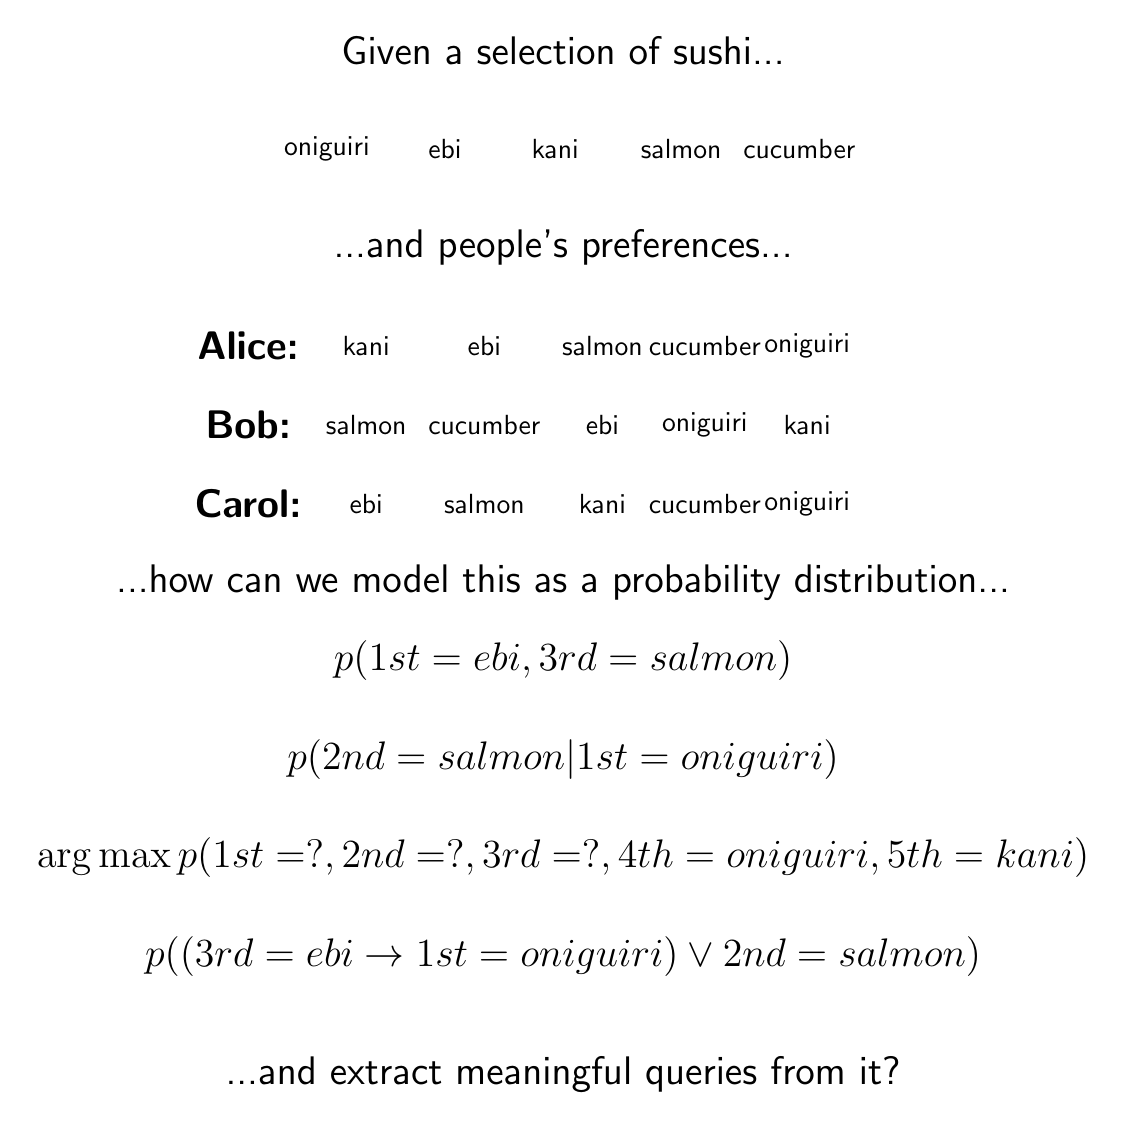
\begin{tikzpicture}
      \node at (3,1.25) {\Large Given a selection of sushi...};

      \node at (0,0) {\sushi{oniguiri}};
      \node at (1.5,0) {\sushi{ebi}};
      \node at (2.9,0) {\sushi{kani}};
      \node at (4.5,0) {\sushi{salmon}};
      \node at (6.0,0) {\sushi{cucumber}};

      \node at (3,-1.25) {\Large{}...and people's preferences...};

      \node (alice) at (-1, -2.5) {\Large\textbf{Alice:}};
      \node (a1) at ($(alice) + (1.5,0)$) {\sushi{kani}};
      \node (a2) at ($(a1) + (1.5,0)$) {\sushi{ebi}};
      \node (a3) at ($(a2) + (1.5,0)$) {\sushi{salmon}};
      \node (a4) at ($(a3) + (1.3,0)$) {\sushi{cucumber}};
      \node (a5) at ($(a4) + (1.3,0.0)$) {\sushi{oniguiri}};

      \node (bob) at ($(alice) + (0,-1)$) {\Large\textbf{Bob:}};
      \node (b1) at ($(a1) + (0,-1)$) {\sushi{salmon}};
      \node (b2) at ($(a2) + (0,-1)$) {\sushi{cucumber}};
      \node (b3) at ($(a3) + (0,-1)$) {\sushi{ebi}};
      \node (b4) at ($(a4) + (0,-1)$) {\sushi{oniguiri}};
      \node (b5) at ($(a5) + (0,-1)$) {\sushi{kani}};

      \node (carol) at ($(bob) + (0,-1)$) {\Large\textbf{Carol:}};
      \node (c1) at ($(b1) + (0,-1)$) {\sushi{ebi}};
      \node (c2) at ($(b2) + (0,-1)$) {\sushi{salmon}};
      \node (c3) at ($(b3) + (0,-1)$) {\sushi{kani}};
      \node (c4) at ($(b4) + (0,-1)$) {\sushi{cucumber}};
      \node (c5) at ($(b5) + (0,-1)$) {\sushi{oniguiri}};

      \node at (3,-5.5) {\Large{}...how can we model this as a probability distribution...};

      \node (q1) at (3,-6.5) {\Large$p(\rankp{1}{st}=\isushi{ebi},\rankp{3}{rd}=\isushi{salmon})$};
      \node (q2) at ($(q1) + (0,-1.25)$) {\Large$p(\rankp{2}{nd}=\isushi{salmon}|\rankp{1}{st}=\isushi{oniguiri})$};
      \node (q3) at ($(q2) + (0,-1.25)$) {\Large$\argmax p(\rankp{1}{st}=?,\rankp{2}{nd}=?,\rankp{3}{rd}=?,\rankp{4}{th}=\isushi{oniguiri},\rankp{5}{th}=\isushi{kani})$};
      \node (q4) at ($(q3) + (0,-1.25)$) {\Large$p((\rankp{3}{rd}=\isushi{ebi}\to\rankp{1}{st}=\isushi{oniguiri})\vee\rankp{2}{nd}=\isushi{salmon})$};

      \node at ($(q4) + (0,-1.5)$) {\Large{}...and extract meaningful queries from it?};
    \end{tikzpicture}
    }
  \end{minipage}
\end{center}

\textcolor{boxdgray}{\cite{kamishima03}}

% Slide: Motivation 2

\newpage

\newtitle{Motivation}
\vspace*{-1cm}

\begin{center}
  \newcommand{\sushi}[1]{\includegraphics[width=32px]{figures/#1}}
  \newcommand{\isushi}[1]{\includegraphics[width=32px,trim=0 75px 0 0]{figures/#1}}
  \newcommand{\rankp}[2]{\text{#1\tsup{#2}}}
  \begin{minipage}{\textwidth}
    \centering
    \resizebox{!}{0.95\textheight}{
    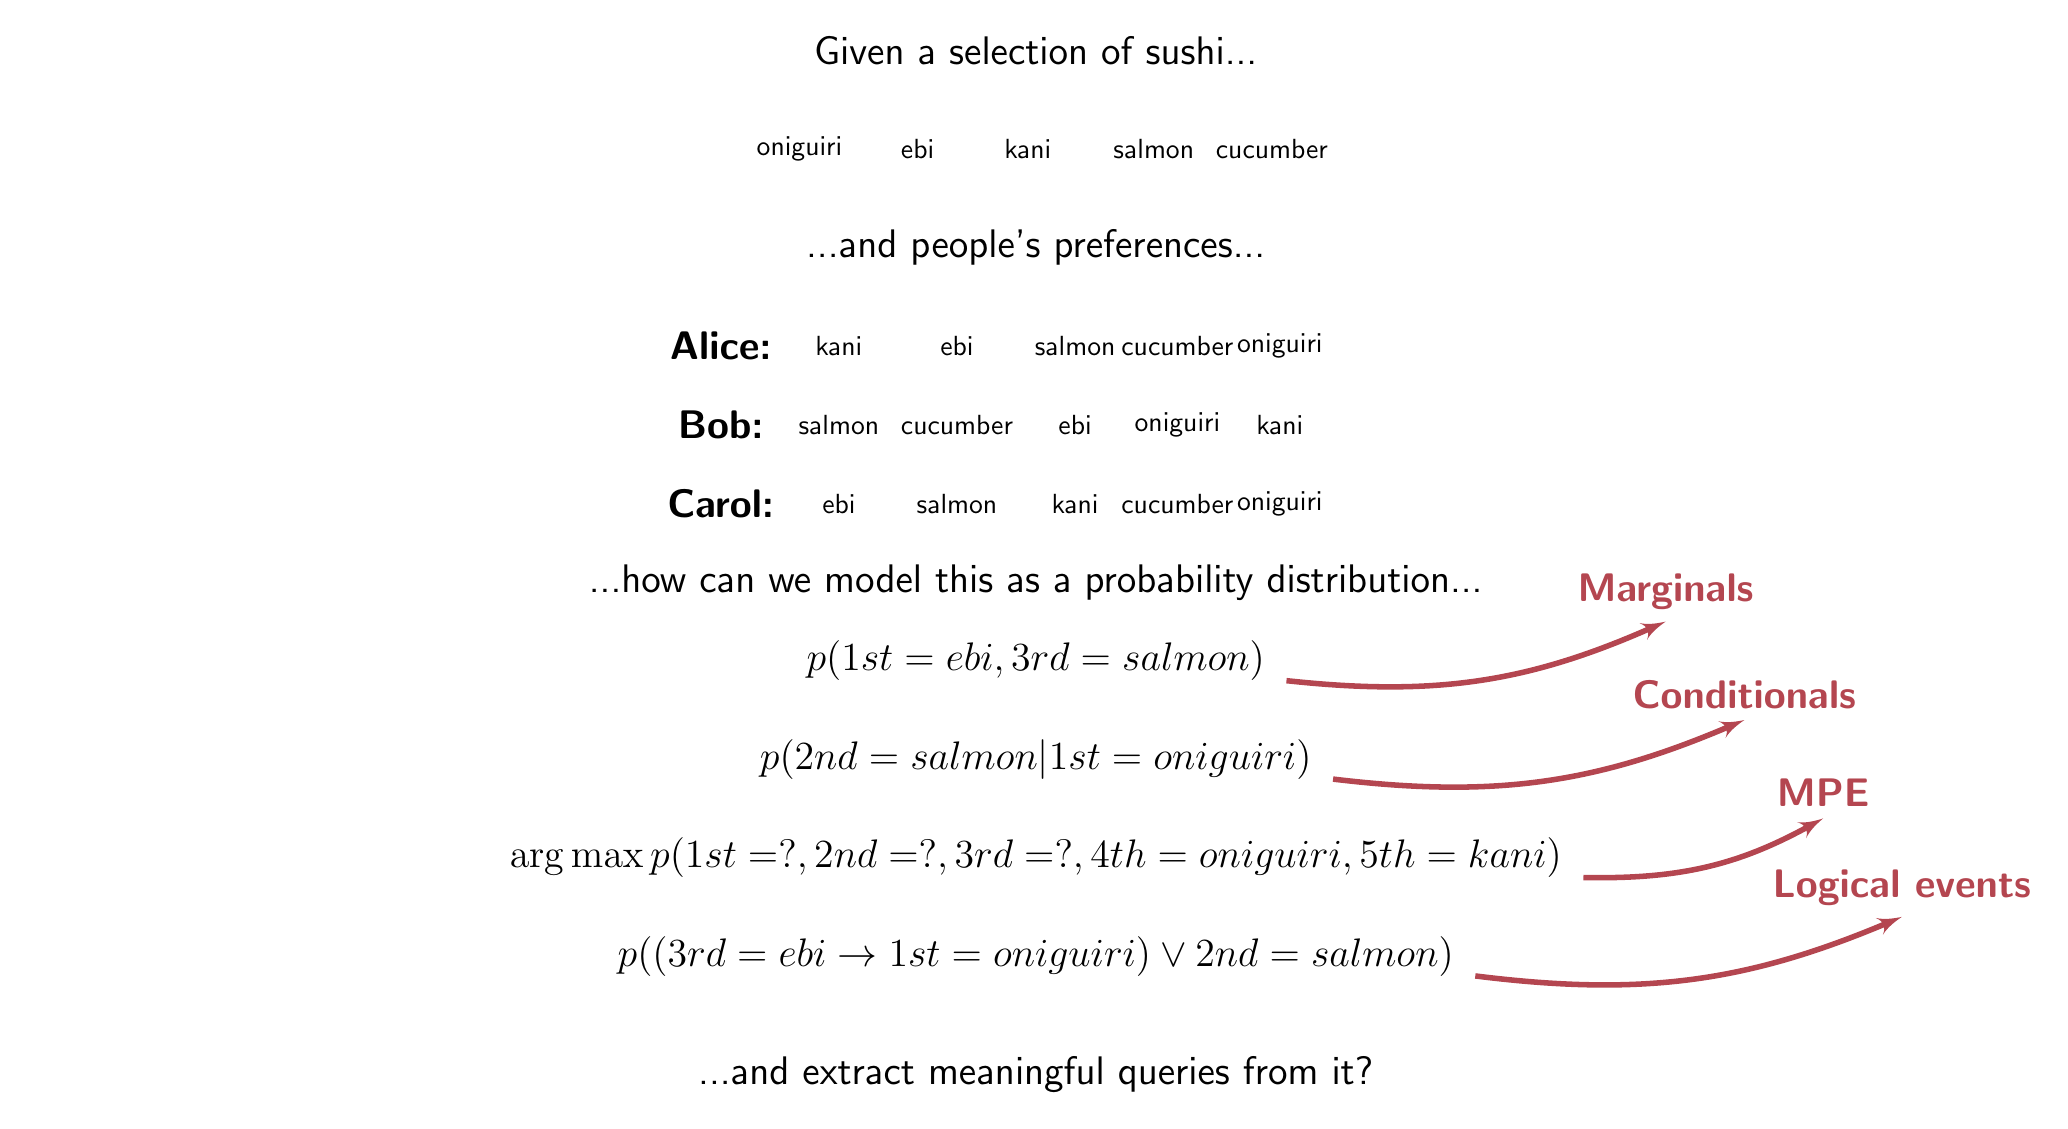
\begin{tikzpicture}
      \node at (3,1.25) {\Large Given a selection of sushi...};

      \node at (0,0) {\sushi{oniguiri}};
      \node at (1.5,0) {\sushi{ebi}};
      \node at (2.9,0) {\sushi{kani}};
      \node at (4.5,0) {\sushi{salmon}};
      \node at (6.0,0) {\sushi{cucumber}};

      \node at (3,-1.25) {\Large{}...and people's preferences...};

      \node (alice) at (-1, -2.5) {\Large\textbf{Alice:}};
      \node (a1) at ($(alice) + (1.5,0)$) {\sushi{kani}};
      \node (a2) at ($(a1) + (1.5,0)$) {\sushi{ebi}};
      \node (a3) at ($(a2) + (1.5,0)$) {\sushi{salmon}};
      \node (a4) at ($(a3) + (1.3,0)$) {\sushi{cucumber}};
      \node (a5) at ($(a4) + (1.3,0.0)$) {\sushi{oniguiri}};

      \node (bob) at ($(alice) + (0,-1)$) {\Large\textbf{Bob:}};
      \node (b1) at ($(a1) + (0,-1)$) {\sushi{salmon}};
      \node (b2) at ($(a2) + (0,-1)$) {\sushi{cucumber}};
      \node (b3) at ($(a3) + (0,-1)$) {\sushi{ebi}};
      \node (b4) at ($(a4) + (0,-1)$) {\sushi{oniguiri}};
      \node (b5) at ($(a5) + (0,-1)$) {\sushi{kani}};

      \node (carol) at ($(bob) + (0,-1)$) {\Large\textbf{Carol:}};
      \node (c1) at ($(b1) + (0,-1)$) {\sushi{ebi}};
      \node (c2) at ($(b2) + (0,-1)$) {\sushi{salmon}};
      \node (c3) at ($(b3) + (0,-1)$) {\sushi{kani}};
      \node (c4) at ($(b4) + (0,-1)$) {\sushi{cucumber}};
      \node (c5) at ($(b5) + (0,-1)$) {\sushi{oniguiri}};

      \node at (3,-5.5) {\Large{}...how can we model this as a probability distribution...};

      \node (q1) at (3,-6.5) {\Large$p(\rankp{1}{st}=\isushi{ebi},\rankp{3}{rd}=\isushi{salmon})$};
      \node (q2) at ($(q1) + (0,-1.25)$) {\Large$p(\rankp{2}{nd}=\isushi{salmon}|\rankp{1}{st}=\isushi{oniguiri})$};
      \node (q3) at ($(q2) + (0,-1.25)$) {\Large$\argmax p(\rankp{1}{st}=?,\rankp{2}{nd}=?,\rankp{3}{rd}=?,\rankp{4}{th}=\isushi{oniguiri},\rankp{5}{th}=\isushi{kani})$};
      \node (q4) at ($(q3) + (0,-1.25)$) {\Large$p((\rankp{3}{rd}=\isushi{ebi}\to\rankp{1}{st}=\isushi{oniguiri})\vee\rankp{2}{nd}=\isushi{salmon})$};

      \draw[edge,line width=2pt,boxred] ($(q1.east) + (0.15,-0.25)$) edge[bend right=15] node[pos=1,above] {\color{boxred}\Large\textbf{Marginals}} ($(q1) + (8,0.5)$);
      \draw[edge,line width=2pt,boxred] ($(q2.east) + (0.15,-0.25)$) edge[bend right=15] node[pos=1,above] {\color{boxred}\Large\textbf{Conditionals}} ($(q2) + (9,0.5)$);
      \draw[edge,line width=2pt,boxred] ($(q3.east) + (0.15,-0.25)$) edge[bend right=15] node[pos=1,above] {\color{boxred}\Large\textbf{MPE}} ($(q3) + (10,0.5)$);
      \draw[edge,line width=2pt,boxred] ($(q4.east) + (0.15,-0.25)$) edge[bend right=15] node[pos=1,above] {\color{boxred}\Large\textbf{Logical events}} ($(q4) + (11,0.5)$);

      \node at ($(q4) + (0,-1.5)$) {\Large{}...and extract meaningful queries from it?};
      \node at ($(q4) + (-11.65,0.5)$) {\phantom{Logical events}};
    \end{tikzpicture}
    }
  \end{minipage}
\end{center}

\textcolor{boxdgray}{\cite{kamishima03}}

\newpage

% Slide: PC - Inputs

\newtitle{Probabilistic Circuits -- Inputs}
\vspace*{0.5cm}

\begin{center}
\begin{minipage}[t][0.8\textheight][t]{0.45\textwidth}
  \begin{vhcenterb}
    \resizebox{\textwidth}{!}{
    \begin{tikzpicture}
      \pgfplotsset{
        every axis/.append style={
          axis line style={->},
          tick label style={font={\scriptsize\bfseries}},
          x tick label style={color=white,above right},
          y tick label style={color=white,above right},
          grid style={black,dashed},
        }
      }
      \begin{axis}[
        no markers, domain=-5:5, samples=35,
        height=3cm, width=5cm,
        xtick={0.8}, ytick={0.29},
        xticklabels={\colorbox{boxblue}{$\mathbf{0.8}$}},
        yticklabels={\colorbox{boxgreen}{$\mathbf{0.29}$}},
        axis lines*=left, xlabel=$x$, ylabel=$p(x)$,
        every axis y label/.style={font=\scriptsize,at={(axis description cs:-0.1,0.9)},anchor=south},
        every axis x label/.style={font=\scriptsize,at=(current axis.right of origin),anchor=west},
        enlargelimits=false, clip=false, axis on top,
        grid = major
      ]
        \path[name path=axis] (axis cs:0,0) -- (axis cs:5,0);
        \addplot[very thick,boxteal,name path=g] {gauss(0,1)};
        \addplot[boxteal!40] fill between [of=g and axis];
      \end{axis}
    \end{tikzpicture}
    }
  \end{vhcenterb}
\end{minipage}
\begin{minipage}[t][0.8\textheight][t]{0.45\textwidth}
  \begin{vhcenterb}
    \resizebox{0.7\textwidth}{!}{
    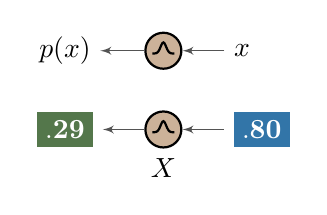
\begin{tikzpicture}
      \node (px) at (0.525, -0.7) {$p(x)$};
      \newGaussNode{g}{$(px) + (1.25,0)$};
      \node (x) at ($(g) + (1,0)$) {$x$};
      \draw[boxdgray,edge] (g) -- (px);
      \draw[boxdgray,edge] (x) -- (g);

      \newGaussNode[label=below:$X$]{gv}{$(g) - (0,1.0)$};
      \node (pxv) at ($(gv) - (1.25,0)$) {\colorbox{boxgreen}{\color{white}$\mathbf{.29}$}};
      \node (xv) at ($(gv) + (1.25,0)$) {\colorbox{boxblue}{\color{white}$\mathbf{.80}$}};
      \draw[boxdgray,edge] (gv) -- (pxv);
      \draw[boxdgray,edge] (xv) -- (gv);
    \end{tikzpicture}
    }
  \end{vhcenterb}
\end{minipage}
\end{center}

% Slide: PC - Sums

\newpage

\newtitle{Probabilistic Circuits -- Sums}
\vspace*{0.5cm}

\begin{center}
\newcommand\mone{1}%
\newcommand\sone{0.65}%
\newcommand\mtwo{2.5}%
\newcommand\stwo{0.85}%
\newcommand\mthr{4}%
\newcommand\sthr{0.6}%
\begin{minipage}[t][0.8\textheight][t]{0.45\textwidth}
  \begin{vhcenterb}
    \resizebox{\textwidth}{!}{
    \begin{tikzpicture}
      \pgfplotsset{
        every axis/.append style={
          axis line style={->},
          tick label style={font={\scriptsize\bfseries}},
          x tick label style={color=white,below},
          y tick label style={color=white,left},
          grid style={black,dashed},
        }
      }
      \begin{axis}[
        no markers, domain=-1:6, samples=35,
        height=3.75cm, width=5cm,
        xtick={1.5}, ytick={0.2414},
        xticklabels={\colorbox{boxblue}{\textbf{1.5}}},
        yticklabels={\colorbox{boxgreen}{\textbf{0.24}}},
        axis lines*=left, xlabel=$x$, ylabel=$p(x)$,
        every axis y label/.style={font=\scriptsize,at={(axis description cs:-0.1,0.9)},anchor=south},
        every axis x label/.style={font=\scriptsize,at=(current axis.right of origin),anchor=west},
        enlargelimits=false, clip=false, axis on top,
        grid = major
      ]
        \path[name path=axis] (axis cs:0,0) -- (axis cs:5,0);
        \addplot[very thick,boxteal,name path=g1] {gauss(\mone,\sone)};
        \addplot[very thick,boxorange,name path=g2] {gauss(\mtwo,\stwo)};
        \addplot[very thick,boxpurple,name path=g3] {gauss(\mthr,\sthr)};
        \addplot[very thick,boxred] {mixgauss3(\mone,\sone,\mtwo,\stwo,\mthr,\sthr,0.4,0.25,0.35)};
        \addplot[boxteal!60] fill between [of=g1 and axis];
        \addplot[boxorange!50] fill between [of=g2 and axis];
        \addplot[boxpurple!40] fill between [of=g3 and axis];
        \node at (\mone, 0.7) {\tiny$\mu_1=\mone$};
        \node at (\mtwo, 0.5) {\tiny$\mu_2=\mtwo$};
        \node at (\mthr, 0.75) {\tiny$\mu_3=\mthr$};
      \end{axis}
    \end{tikzpicture}
    }
  \end{vhcenterb}
\end{minipage}
\begin{minipage}[t][0.8\textheight][t]{0.45\textwidth}
  \begin{vhcenterb}
    \resizebox{0.7\textwidth}{!}{
    \begin{tikzpicture}
      \newSumNode[fill=boxred!70]{s}{0,0};
      \newGaussNode[fill=boxteal]{g1}{$(s) + (-1.5,-1)$};
      \newGaussNode[fill=boxorange!80]{g2}{$(s) + (0,-1)$};
      \newGaussNode[fill=boxpurple!60]{g3}{$(s) + (1.5,-1)$};
      \draw[edge] (s) edge (g1);
      \draw[edge] (s) edge (g2);
      \draw[edge] (s) edge (g3);
      \node at ($(s) + (-1.2,-0.35)$) {\scriptsize$.40$};
      \node at ($(s) + (-0.3,-0.5)$) {\scriptsize$.25$};
      \node at ($(s) + (1,-0.35)$) {\scriptsize$.35$};
      \node (l1) at ($(g1) + (0,-0.5)$) {\scriptsize$\gaussian_1(\mone,\sone)$};
      \node (l2) at ($(g2) + (0,-0.5)$) {\scriptsize$\gaussian_2(\mtwo,\stwo)$};
      \node (l3) at ($(g3) + (0,-0.5)$) {\scriptsize$\gaussian_3(\mthr,\sthr)$};
    \end{tikzpicture}
    }
    \resizebox{0.7\textwidth}{!}{
    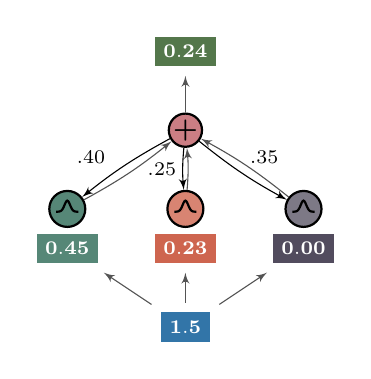
\begin{tikzpicture}
      \newSumNode[fill=boxred!70]{s}{0,0};
      \newGaussNode[fill=boxteal]{g1}{$(s) + (-1.5,-1)$};
      \newGaussNode[fill=boxorange!80]{g2}{$(s) + (0,-1)$};
      \newGaussNode[fill=boxpurple!60]{g3}{$(s) + (1.5,-1)$};
      \draw[edge] (s) edge[bend right=5] (g1);
      \draw[edge] (s) edge[bend right=5] (g2);
      \draw[edge] (s) edge[bend right=5] (g3);
      \node at ($(s) + (-1.2,-0.35)$) {\scriptsize$.40$};
      \node at ($(s) + (-0.3,-0.5)$) {\scriptsize$.25$};
      \node at ($(s) + (1,-0.35)$) {\scriptsize$.35$};
      \node (inp) at ($(g2) + (0,-1.5)$) {\scriptsize\colorbox{boxblue}{\color{white}$\mathbf{1.5}$}};
      \node (out) at ($(s) + (0,1.0)$) {\scriptsize\colorbox{boxgreen}{\color{white}$\mathbf{0.24}$}};
      \draw[edge,boxdgray] (s) -- (out);
      \node (l1) at ($(g1) + (0,-0.5)$) {\scriptsize\colorbox{boxteal}{\color{white}$\mathbf{0.45}$}};
      \node (l2) at ($(g2) + (0,-0.5)$) {\scriptsize\colorbox{boxorange}{\color{white}$\mathbf{0.23}$}};
      \node (l3) at ($(g3) + (0,-0.5)$) {\scriptsize\colorbox{boxpurple!80}{\color{white}$\mathbf{0.00}$}};
      \draw[edge,boxdgray] (inp) edge (l1);
      \draw[edge,boxdgray] (inp) edge (l2);
      \draw[edge,boxdgray] (inp) edge (l3);
      \draw[edge,boxdgray] (g1) edge[bend left=-5] (s);
      \draw[edge,boxdgray] (g2) edge[bend left=-5] (s);
      \draw[edge,boxdgray] (g3) edge[bend left=-5] (s);
    \end{tikzpicture}
    }
  \end{vhcenterb}
\end{minipage}
\end{center}

% Slide: PC - Smoothness

\newpage

\newtitle{Probabilistic Circuits -- Smoothness}
\vspace*{0.5cm}

\begin{center}
\newcommand\mone{1}%
\newcommand\sone{0.65}%
\newcommand\mtwo{2.5}%
\newcommand\stwo{0.85}%
\newcommand\mthr{4}%
\newcommand\sthr{0.6}%
\begin{minipage}[t][0.8\textheight][t]{0.45\textwidth}
  \begin{vhcenterb}
    \resizebox{\textwidth}{!}{
    \begin{tikzpicture}
      \pgfplotsset{
        every axis/.append style={
          axis line style={->},
          tick label style={font={\scriptsize\bfseries}},
          x tick label style={color=white,below},
          y tick label style={color=white,left},
          grid style={black,dashed},
        }
      }
      \begin{axis}[
        no markers, domain=-1:6, samples=35,
        height=3.75cm, width=5cm,
        xtick={1.5}, ytick={0.2414},
        xticklabels={\colorbox{boxblue}{\textbf{1.5}}},
        yticklabels={\colorbox{boxgreen}{\textbf{0.24}}},
        axis lines*=left, xlabel=$x$, ylabel=$p(x)$,
        every axis y label/.style={font=\scriptsize,at={(axis description cs:-0.1,0.9)},anchor=south},
        every axis x label/.style={font=\scriptsize,at=(current axis.right of origin),anchor=west},
        enlargelimits=false, clip=false, axis on top,
        grid = major
      ]
        \path[name path=axis] (axis cs:0,0) -- (axis cs:5,0);
        \addplot[very thick,boxteal,name path=g1] {gauss(\mone,\sone)};
        \addplot[very thick,boxorange,name path=g2] {gauss(\mtwo,\stwo)};
        \addplot[very thick,boxpurple,name path=g3] {gauss(\mthr,\sthr)};
        \addplot[very thick,boxred] {mixgauss3(\mone,\sone,\mtwo,\stwo,\mthr,\sthr,0.4,0.25,0.35)};
        \addplot[boxteal!60] fill between [of=g1 and axis];
        \addplot[boxorange!50] fill between [of=g2 and axis];
        \addplot[boxpurple!40] fill between [of=g3 and axis];
        \node at (\mone, 0.7) {\tiny$X$};
        \node at (\mtwo, 0.55) {\tiny$X$};
        \node at (\mthr, 0.75) {\tiny$X$};
      \end{axis}
    \end{tikzpicture}
    }
    \vskip 0.5cm
    \resizebox{\textwidth}{!}{\begin{minipage}{0.675\textwidth}
      \begin{definition}[Smoothness]~\\
        Every sum node child mentions the \underline{same} variables.
      \end{definition}
    \end{minipage}}
  \end{vhcenterb}
\end{minipage}
\begin{minipage}[t][0.8\textheight][t]{0.45\textwidth}
  \begin{vhcenterb}
    \resizebox{0.7\textwidth}{!}{
    \begin{tikzpicture}
      \newSumNode[fill=boxred!70]{s}{0,0};
      \newGaussNode[fill=boxteal]{g1}{$(s) + (-1.5,-1)$};
      \newGaussNode[fill=boxorange!80]{g2}{$(s) + (0,-1)$};
      \newGaussNode[fill=boxpurple!60]{g3}{$(s) + (1.5,-1)$};
      \draw[edge] (s) edge (g1);
      \draw[edge] (s) edge (g2);
      \draw[edge] (s) edge (g3);
      \node at ($(s) + (-1.2,-0.35)$) {\scriptsize$.40$};
      \node at ($(s) + (-0.3,-0.5)$) {\scriptsize$.25$};
      \node at ($(s) + (1,-0.35)$) {\scriptsize$.35$};
      \node (l1) at ($(g1) + (0,-0.5)$) {\scriptsize$\gaussian_1(\mone,\sone)$};
      \node (l2) at ($(g2) + (0,-0.5)$) {\scriptsize$\gaussian_2(\mtwo,\stwo)$};
      \node (l3) at ($(g3) + (0,-0.5)$) {\scriptsize$\gaussian_3(\mthr,\sthr)$};
    \end{tikzpicture}
    }
    \resizebox{0.65\textwidth}{!}{
    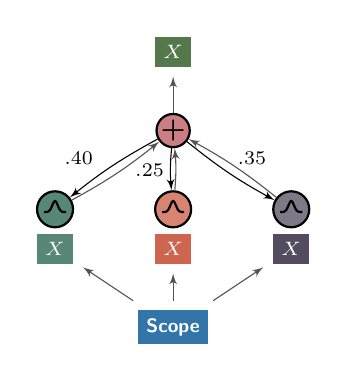
\begin{tikzpicture}
      \newSumNode[fill=boxred!70]{s}{0,0};
      \newGaussNode[fill=boxteal]{g1}{$(s) + (-1.5,-1)$};
      \newGaussNode[fill=boxorange!80]{g2}{$(s) + (0,-1)$};
      \newGaussNode[fill=boxpurple!60]{g3}{$(s) + (1.5,-1)$};
      \draw[edge] (s) edge[bend right=5] (g1);
      \draw[edge] (s) edge[bend right=5] (g2);
      \draw[edge] (s) edge[bend right=5] (g3);
      \node at ($(s) + (-1.2,-0.35)$) {\scriptsize$.40$};
      \node at ($(s) + (-0.3,-0.5)$) {\scriptsize$.25$};
      \node at ($(s) + (1,-0.35)$) {\scriptsize$.35$};
      \node (inp) at ($(g2) + (0,-1.5)$) {\scriptsize\colorbox{boxblue}{\color{white}\textbf{Scope}}};
      \node (out) at ($(s) + (0,1.0)$) {\scriptsize\colorbox{boxgreen}{\color{white}$X$}};
      \draw[edge,boxdgray] (s) -- (out);
      \node (l1) at ($(g1) + (0,-0.5)$) {\scriptsize\colorbox{boxteal}{\color{white}$X$}};
      \node (l2) at ($(g2) + (0,-0.5)$) {\scriptsize\colorbox{boxorange}{\color{white}$X$}};
      \node (l3) at ($(g3) + (0,-0.5)$) {\scriptsize\colorbox{boxpurple!80}{\color{white}$X$}};
      \draw[edge,boxdgray] (inp) edge (l1);
      \draw[edge,boxdgray] (inp) edge (l2);
      \draw[edge,boxdgray] (inp) edge (l3);
      \draw[edge,boxdgray] (g1) edge[bend left=-5] (s);
      \draw[edge,boxdgray] (g2) edge[bend left=-5] (s);
      \draw[edge,boxdgray] (g3) edge[bend left=-5] (s);
    \end{tikzpicture}
    }
  \end{vhcenterb}
\end{minipage}
\end{center}

\textcolor{boxdgray}{\cite{darwiche01a}}

% Slide: PC - Determinism

\newpage

\newtitle{Probabilistic Circuits -- Determinism}
\vspace*{0.5cm}

\begin{center}
\newcommand\mone{1}%
\newcommand\sone{0.65}%
\newcommand\mtwo{2.5}%
\newcommand\stwo{0.85}%
\newcommand\mthr{4}%
\newcommand\sthr{0.6}%
\begin{minipage}[t][0.8\textheight][t]{0.45\textwidth}
  \begin{vhcenterb}
    \resizebox{\textwidth}{!}{
    \begin{tikzpicture}
      \pgfplotsset{
        every axis/.append style={
          axis line style={->},
          tick label style={font={\scriptsize\bfseries}},
          x tick label style={color=white,below},
          y tick label style={color=white,left},
          grid style={black,dashed},
        }
      }
      \begin{axis}[
        no markers, domain=-1:6, samples=35,
        height=3.75cm, width=5cm,
        xtick={1.5}, ytick={0.07753},
        xticklabels={\colorbox{boxblue}{\textbf{1.5}}},
        yticklabels={\colorbox{boxgreen}{\textbf{0.07}}},
        axis lines*=left, xlabel=$x$, ylabel=$p(x)$,
        every axis y label/.style={font=\scriptsize,at={(axis description cs:-0.1,0.9)},anchor=south},
        every axis x label/.style={font=\scriptsize,at=(current axis.right of origin),anchor=west},
        enlargelimits=false, clip=false, axis on top,
        grid = major
      ]
        \path[name path=axis] (axis cs:0,0) -- (axis cs:5,0);
        \addplot[domain=-1:1.25,very thick,boxteal,name path=g1] {gauss(\mone,\sone)};
        \draw[very thick,boxteal] (1.25,0.572) -- (1.25,0.1591);
        \addplot[domain=1.25:3.25,very thick,boxorange,name path=g2] {gauss(\mtwo,\stwo)};
        \addplot[domain=3.25:6,very thick,boxpurple,name path=g3] {gauss(\mthr,\sthr)};
        \addplot[very thick,boxred] {mixgauss3t(\mone,\sone,\mtwo,\stwo,\mthr,\sthr,0.4,0.25,0.35)};
        \addplot[boxteal!60] fill between [of=g1 and axis, soft clip={domain=-1:1.25}];
        \addplot[boxorange!50] fill between [of=g2 and axis, soft clip={domain=1.25:3.25}];
        \addplot[boxpurple!40] fill between [of=g3 and axis, soft clip={domain=3.25:6}];
        \node at (\mone, 0.7) {\tiny$X$};
        \node at (\mtwo, 0.55) {\tiny$X$};
        \node at (\mthr, 0.75) {\tiny$X$};
      \end{axis}
    \end{tikzpicture}
    }
    \vskip 0.5cm
    \resizebox{\textwidth}{!}{\begin{minipage}{0.675\textwidth}
      \begin{definition}[Determinism]~\\
        \underline{At most one} sum node child has a positive value.
      \end{definition}
    \end{minipage}}
  \end{vhcenterb}
\end{minipage}
\begin{minipage}[t][0.8\textheight][t]{0.45\textwidth}
  \begin{vhcenterb}
    \resizebox{0.7\textwidth}{!}{
    \begin{tikzpicture}
      \newSumNode[fill=boxred!70]{s}{0,0};
      \newGaussNode[fill=boxteal]{g1}{$(s) + (-1.5,-1)$};
      \newGaussNode[fill=boxorange!80]{g2}{$(s) + (0,-1)$};
      \newGaussNode[fill=boxpurple!60]{g3}{$(s) + (1.5,-1)$};
      \draw[edge] (s) edge (g1);
      \draw[edge] (s) edge (g2);
      \draw[edge] (s) edge (g3);
      \node at ($(s) + (-1.2,-0.35)$) {\scriptsize$.40$};
      \node at ($(s) + (-0.3,-0.5)$) {\scriptsize$.25$};
      \node at ($(s) + (1,-0.35)$) {\scriptsize$.35$};
      \node (l1) at ($(g1) + (0,-0.5)$) {\scriptsize$\Psi_1(\mone,\sone)$};
      \node (l2) at ($(g2) + (0,-0.5)$) {\scriptsize$\Psi_2(\mtwo,\stwo)$};
      \node (l3) at ($(g3) + (0,-0.5)$) {\scriptsize$\Psi_3(\mthr,\sthr)$};
    \end{tikzpicture}
    }
    \resizebox{0.7\textwidth}{!}{
    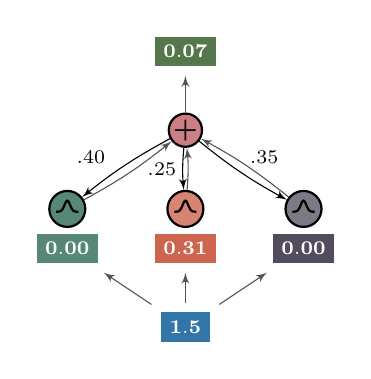
\begin{tikzpicture}
      \newSumNode[fill=boxred!70]{s}{0,0};
      \newGaussNode[fill=boxteal]{g1}{$(s) + (-1.5,-1)$};
      \newGaussNode[fill=boxorange!80]{g2}{$(s) + (0,-1)$};
      \newGaussNode[fill=boxpurple!60]{g3}{$(s) + (1.5,-1)$};
      \draw[edge] (s) edge[bend right=5] (g1);
      \draw[edge] (s) edge[bend right=5] (g2);
      \draw[edge] (s) edge[bend right=5] (g3);
      \node at ($(s) + (-1.2,-0.35)$) {\scriptsize$.40$};
      \node at ($(s) + (-0.3,-0.5)$) {\scriptsize$.25$};
      \node at ($(s) + (1,-0.35)$) {\scriptsize$.35$};
      \node (inp) at ($(g2) + (0,-1.5)$) {\scriptsize\colorbox{boxblue}{\color{white}$\mathbf{1.5}$}};
      \node (out) at ($(s) + (0,1.0)$) {\scriptsize\colorbox{boxgreen}{\color{white}$\mathbf{0.07}$}};
      \draw[edge,boxdgray] (s) -- (out);
      \node (l1) at ($(g1) + (0,-0.5)$) {\scriptsize\colorbox{boxteal}{\color{white}$\mathbf{0.00}$}};
      \node (l2) at ($(g2) + (0,-0.5)$) {\scriptsize\colorbox{boxorange}{\color{white}$\mathbf{0.31}$}};
      \node (l3) at ($(g3) + (0,-0.5)$) {\scriptsize\colorbox{boxpurple!80}{\color{white}$\mathbf{0.00}$}};
      \draw[edge,boxdgray] (inp) edge (l1);
      \draw[edge,boxdgray] (inp) edge (l2);
      \draw[edge,boxdgray] (inp) edge (l3);
      \draw[edge,boxdgray] (g1) edge[bend left=-5] (s);
      \draw[edge,boxdgray] (g2) edge[bend left=-5] (s);
      \draw[edge,boxdgray] (g3) edge[bend left=-5] (s);
    \end{tikzpicture}
    }
  \end{vhcenterb}
\end{minipage}
\end{center}

\textcolor{boxdgray}{\cite{darwiche01a}}

% Slide: PC - Products

\newpage

\newtitle{Probabilistic Circuits -- Products}
\vspace*{0.25cm}

\begin{center}
\newcommand\xmone{2}%
\newcommand\xsone{0.5}%
\newcommand\xmtwo{4}%
\newcommand\xstwo{0.8}%
\newcommand\ymone{3}%
\newcommand\ysone{0.7}%
\newcommand\ymtwo{5}%
\newcommand\ystwo{0.4}%
\begin{minipage}[t][0.8\textheight][t]{0.45\textwidth}
  \begin{vhcenterb}
    \resizebox{\textwidth}{!}{
    \begin{tikzpicture}
      \pgfplotsset{
        every axis/.append style={
          axis line style={->},
          tick label style={font={\scriptsize\bfseries}},
          x tick label style={color=white,below},
          y tick label style={color=white,left},
          grid style={black,dashed},
        }
      }
      \begin{axis}[
        no markers, domain=0:7, samples=35,
        width=5cm, height=3.5cm,
        xtick={2}, ytick={0.25},
        xticklabels={\colorbox{boxblue}{\textbf{2}}},
        yticklabels={\colorbox{boxred}{\textbf{0.25}}},
        axis lines*=left, xlabel=$x$, ylabel=$p(x)$,
        every axis y label/.style={font=\scriptsize,at={(axis description cs:-0.1,0.9)},anchor=south},
        every axis x label/.style={font=\scriptsize,at=(current axis.right of origin),anchor=west},
        enlargelimits=false, clip=false, axis on top,
        grid = major
      ]
        \path[name path=axis] (axis cs:0,0) -- (axis cs:7,0);
        \addplot[very thick,boxteal,name path=g1] {gauss(\xmone,\xsone)};
        \addplot[very thick,boxorange,name path=g2] {gauss(\xmtwo,\xstwo)};
        \addplot[very thick,boxred] {mixgauss2(\xmone,\xsone,\xmtwo,\xstwo,0.3,0.7)};
        \addplot[boxteal!60] fill between [of=g1 and axis];
        \addplot[boxorange!50] fill between [of=g2 and axis];
        \node at (axis cs:\xmone,{egauss(\xmone,\xsone,\xmone)+0.1}) {\tiny$\mu_1=\xmone$};
        \node at (axis cs:\xmtwo,{egauss(\xmtwo,\xstwo,\xmtwo)+0.1}) {\tiny$\mu_2=\xmtwo$};
      \end{axis}
    \end{tikzpicture}
    \begin{tikzpicture}
      \pgfplotsset{
        every axis/.append style={
          axis line style={->},
          tick label style={font={\scriptsize\bfseries}},
          x tick label style={color=white,below},
          y tick label style={color=white,left},
          grid style={black,dashed},
        }
      }
      \begin{axis}[
        no markers, domain=1:7, samples=50,
        width=5cm, height=3.5cm,
        xtick={4}, ytick={0.14},
        xticklabels={\colorbox{boxblue}{\textbf{4}}},
        yticklabels={\colorbox{boxpurple}{\textbf{0.14}}},
        axis lines*=left, xlabel=$y$, ylabel=$p(y)$,
        every axis y label/.style={font=\scriptsize,at={(axis description cs:-0.1,0.9)},anchor=south},
        every axis x label/.style={font=\scriptsize,at=(current axis.right of origin),anchor=west},
        enlargelimits=false, clip=false, axis on top,
        grid = major
      ]
        \path[name path=axis] (axis cs:0,0) -- (axis cs:7,0);
        \addplot[very thick,boxpink,name path=g1] {gauss(\ymone,\ysone)};
        \addplot[very thick,boxgoldenrod,name path=g2] {gauss(\ymtwo,\ystwo)};
        \addplot[very thick,boxpurple] {mixgauss2(\ymone,\ysone,\ymtwo,\ystwo,0.6,0.4)};
        \addplot[boxpink!40] fill between [of=g1 and axis];
        \addplot[boxgoldenrod!50] fill between [of=g2 and axis];
        \node at (axis cs:\ymone,{egauss(\ymone,\ysone,\ymone)+0.1}) {\tiny$\mu_3=\ymone$};
        \node at (axis cs:\ymtwo,{egauss(\ymtwo,\ystwo,\ymtwo)+0.1}) {\tiny$\mu_4=\ymtwo$};
      \end{axis}
    \end{tikzpicture}
    }
    \begin{tikzpicture}
      \pgfplotsset{
        every axis/.append style={
          axis line style={->},
          axis lines=center,
          grid style={black,dashed},
          x tick label style={color=white,below},
          y tick label style={color=white,right},
          z tick label style={color=white,left},
        }
      }
      \begin{axis}[
        no markers, width=0.8\columnwidth,
        xtick={2}, ytick={4}, ztick={0.035},
        xticklabels={\colorbox{boxblue}{\textbf{2}}},
        yticklabels={\colorbox{boxblue}{\textbf{4}}},
        zticklabels={\colorbox{boxgreen}{\textbf{0.035}}},
        xlabel=$x$, ylabel=$y$, zlabel={$p(x,y)$},
        axis lines*=left,
        xlabel style={anchor=north west},
        ylabel style={anchor=south west},
        zlabel style={anchor=south west},
        enlargelimits=false, clip=false, axis on top,
        grid = major
      ]
        \addplot3[
          surf, samples=30,
          domain=0.5:6.5,
          y domain=1:6
        ] {((0.3*exp(-((x-\xmone)^2)/(2*\xsone^2))/\xsone+0.7*exp(-((x-\xmtwo)^2)/(2*\xstwo^2))/\xstwo)/2.5066)*(((0.6*exp(-((y-\ymone)^2)/(2*\ysone^2))/\ysone+0.4*exp(-((y-\ymtwo)^2)/(2*\ystwo^2))/\ystwo)/2.5066))};
      \end{axis}
    \end{tikzpicture}
  \end{vhcenterb}
\end{minipage}
\begin{minipage}[t][0.8\textheight][t]{0.45\textwidth}
  \begin{vhcenterb}
    \resizebox{0.7\textwidth}{!}{
    \begin{tikzpicture}
      \newProdNode[fill=boxgreen]{r}{0,0};
      \newSumNode[fill=boxred!70]{p}{$(r) + (-1.25,-0.75)$};
      \newSumNode[fill=boxpurple!60]{q}{$(r) + (1.25,-0.75)$};
      \newGaussNode[fill=boxteal]{x1}{$(p) + (-0.6,-1)$};
      \newGaussNode[fill=boxorange!80]{x2}{$(p) + (0.65,-1)$};
      \newGaussNode[fill=boxpink!50]{y1}{$(q) + (-0.6,-1)$};
      \newGaussNode[fill=boxgoldenrod!70]{y2}{$(q) + (0.6,-1)$};
      \draw[edge] (r) edge (p);
      \draw[edge] (r) edge (q);
      \draw[edge] (p) edge (x1);
      \draw[edge] (p) edge (x2);
      \draw[edge] (q) edge (y1);
      \draw[edge] (q) edge (y2);
      \node at ($(p) + (-0.5,-0.4)$) {\scriptsize$.3$};
      \node at ($(p) + (0.5,-0.4)$) {\scriptsize$.7$};
      \node at ($(q) + (-0.5,-0.4)$) {\scriptsize$.6$};
      \node at ($(q) + (0.5,-0.4)$) {\scriptsize$.4$};
      \node (l1) at ($(x1) + (0,-0.5)$) {\scriptsize$\gaussian_1(\xmone,\xsone)$};
      \node (l2) at ($(x2) + (0,-0.5)$) {\scriptsize$\gaussian_2(\xmtwo,\xstwo)$};
      \node (l3) at ($(y1) + (0,-0.5)$) {\scriptsize$\gaussian_3(\ymone,\ysone)$};
      \node (l4) at ($(y2) + (0,-0.5)$) {\scriptsize$\gaussian_4(\ymtwo,\ystwo)$};
    \end{tikzpicture}
    }
    \resizebox{0.7\textwidth}{!}{
    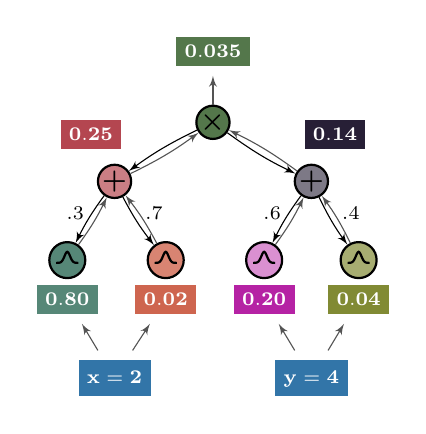
\begin{tikzpicture}
      \newProdNode[fill=boxgreen]{r}{0,0};
      \newSumNode[fill=boxred!70]{p}{$(r) + (-1.25,-0.75)$};
      \newSumNode[fill=boxpurple!60]{q}{$(r) + (1.25,-0.75)$};
      \newGaussNode[fill=boxteal]{x1}{$(p) + (-0.6,-1)$};
      \newGaussNode[fill=boxorange!80]{x2}{$(p) + (0.65,-1)$};
      \newGaussNode[fill=boxpink!50]{y1}{$(q) + (-0.6,-1)$};
      \newGaussNode[fill=boxgoldenrod!70]{y2}{$(q) + (0.6,-1)$};
      \draw[edge] (r) edge[bend right=5] (p);
      \draw[edge] (r) edge[bend right=5] (q);
      \draw[edge] (p) edge[bend right=5] (x1);
      \draw[edge] (p) edge[bend right=5] (x2);
      \draw[edge] (q) edge[bend right=5] (y1);
      \draw[edge] (q) edge[bend right=5] (y2);
      \node at ($(p) + (-0.5,-0.4)$) {\scriptsize$.3$};
      \node at ($(p) + (0.5,-0.4)$) {\scriptsize$.7$};
      \node at ($(q) + (-0.5,-0.4)$) {\scriptsize$.6$};
      \node at ($(q) + (0.5,-0.4)$) {\scriptsize$.4$};
      \node (l1) at ($(x1) + (0,-0.5)$) {\scriptsize\colorbox{boxteal}{\color{white}$\mathbf{0.80}$}};
      \node (l2) at ($(x2) + (0,-0.5)$) {\scriptsize\colorbox{boxorange}{\color{white}$\mathbf{0.02}$}};
      \node (l3) at ($(y1) + (0,-0.5)$) {\scriptsize\colorbox{boxpink}{\color{white}$\mathbf{0.20}$}};
      \node (l4) at ($(y2) + (0,-0.5)$) {\scriptsize\colorbox{boxgoldenrod}{\color{white}$\mathbf{0.04}$}};
      \draw[edge,boxdgray] (p) edge[bend left=-5] (r);
      \draw[edge,boxdgray] (q) edge[bend left=-5] (r);
      \draw[edge,boxdgray] (x1) edge[bend left=-5] (p);
      \draw[edge,boxdgray] (x2) edge[bend left=-5] (p);
      \draw[edge,boxdgray] (y1) edge[bend left=-5] (q);
      \draw[edge,boxdgray] (y2) edge[bend left=-5] (q);
      \node at ($(p) + (-0.3,0.6)$) {\scriptsize\colorbox{boxred}{\color{white}$\mathbf{0.25}$}};
      \node at ($(q) + (0.3,0.6)$) {\scriptsize\colorbox{boxpurple}{\color{white}$\mathbf{0.14}$}};
      \node (x) at ($(p) + (0,-2.5)$) {\scriptsize\colorbox{boxblue}{\color{white}$\mathstrut\mathbf{x=2}$}};
      \node (y) at ($(q) + (0,-2.5)$) {\scriptsize\colorbox{boxblue}{\color{white}$\mathstrut\mathbf{y=4}$}};
      \draw[edge,boxdgray] (x) edge (l1);
      \draw[edge,boxdgray] (x) edge (l2);
      \draw[edge,boxdgray] (y) edge (l3);
      \draw[edge,boxdgray] (y) edge (l4);
      \node (out) at ($(r) + (0,0.9)$) {\scriptsize\colorbox{boxgreen}{\color{white}$\mathbf{0.035}$}};
      \draw[edge,boxdgray] (r) edge (out);
    \end{tikzpicture}
    }
  \end{vhcenterb}
\end{minipage}
\end{center}

% Slide: PC - Decomposabilty

\newpage

\newtitle{Probabilistic Circuits -- Decomposability}
\vspace*{0.25cm}

\begin{center}
\newcommand\xmone{2}%
\newcommand\xsone{0.5}%
\newcommand\xmtwo{4}%
\newcommand\xstwo{0.8}%
\newcommand\ymone{3}%
\newcommand\ysone{0.7}%
\newcommand\ymtwo{5}%
\newcommand\ystwo{0.4}%
\begin{minipage}[t][0.8\textheight][t]{0.45\textwidth}
  \begin{vhcenterb}
    \resizebox{\textwidth}{!}{
    \begin{tikzpicture}
      \pgfplotsset{
        every axis/.append style={
          axis line style={->},
          tick label style={font={\scriptsize\bfseries}},
          x tick label style={color=white,below},
          y tick label style={color=white,left},
          grid style={black,dashed},
        }
      }
      \begin{axis}[
        no markers, domain=0:7, samples=35,
        width=5cm, height=4.0cm,
        xtick={2}, ytick={0.25},
        xticklabels={\colorbox{boxblue}{\textbf{2}}},
        yticklabels={\colorbox{boxred}{\textbf{0.25}}},
        axis lines*=left, xlabel=$x$, ylabel=$p(x)$,
        every axis y label/.style={font=\scriptsize,at={(axis description cs:-0.1,0.9)},anchor=south},
        every axis x label/.style={font=\scriptsize,at=(current axis.right of origin),anchor=west},
        enlargelimits=false, clip=false, axis on top,
        grid = major
      ]
        \path[name path=axis] (axis cs:0,0) -- (axis cs:7,0);
        \addplot[very thick,boxteal,name path=g1] {gauss(\xmone,\xsone)};
        \addplot[very thick,boxorange,name path=g2] {gauss(\xmtwo,\xstwo)};
        \addplot[very thick,boxred] {mixgauss2(\xmone,\xsone,\xmtwo,\xstwo,0.3,0.7)};
        \addplot[boxteal!60] fill between [of=g1 and axis];
        \addplot[boxorange!50] fill between [of=g2 and axis];
        \node at (axis cs:\xmone,{egauss(\xmone,\xsone,\xmone)+0.1}) {\tiny$X$};
        \node at (axis cs:\xmtwo,{egauss(\xmtwo,\xstwo,\xmtwo)+0.1}) {\tiny$X$};
      \end{axis}
    \end{tikzpicture}
    \begin{tikzpicture}
      \pgfplotsset{
        every axis/.append style={
          axis line style={->},
          tick label style={font={\scriptsize\bfseries}},
          x tick label style={color=white,below},
          y tick label style={color=white,left},
          grid style={black,dashed},
        }
      }
      \begin{axis}[
        no markers, domain=1:7, samples=50,
        width=5cm, height=4.0cm,
        xtick={4}, ytick={0.14},
        xticklabels={\colorbox{boxblue}{\textbf{4}}},
        yticklabels={\colorbox{boxpurple}{\textbf{0.14}}},
        axis lines*=left, xlabel=$y$, ylabel=$p(y)$,
        every axis y label/.style={font=\scriptsize,at={(axis description cs:-0.1,0.9)},anchor=south},
        every axis x label/.style={font=\scriptsize,at=(current axis.right of origin),anchor=west},
        enlargelimits=false, clip=false, axis on top,
        grid = major
      ]
        \path[name path=axis] (axis cs:0,0) -- (axis cs:7,0);
        \addplot[very thick,boxpink,name path=g1] {gauss(\ymone,\ysone)};
        \addplot[very thick,boxgoldenrod,name path=g2] {gauss(\ymtwo,\ystwo)};
        \addplot[very thick,boxpurple] {mixgauss2(\ymone,\ysone,\ymtwo,\ystwo,0.6,0.4)};
        \addplot[boxpink!40] fill between [of=g1 and axis];
        \addplot[boxgoldenrod!50] fill between [of=g2 and axis];
        \node at (axis cs:\ymone,{egauss(\ymone,\ysone,\ymone)+0.1}) {\tiny$Y$};
        \node at (axis cs:\ymtwo,{egauss(\ymtwo,\ystwo,\ymtwo)+0.1}) {\tiny$Y$};
      \end{axis}
    \end{tikzpicture}
    }
    \vskip 1.0cm
    \resizebox{\textwidth}{!}{\begin{minipage}{0.675\textwidth}
      \begin{definition}[Decomposability]~\\
        Every product node child mentions \underline{different} variables.
      \end{definition}
    \end{minipage}}
  \end{vhcenterb}
\end{minipage}
\begin{minipage}[t][0.8\textheight][t]{0.45\textwidth}
  \begin{vhcenterb}
    \resizebox{0.7\textwidth}{!}{
    \begin{tikzpicture}
      \newProdNode[fill=boxgreen]{r}{0,0};
      \newSumNode[fill=boxred!70]{p}{$(r) + (-1.25,-0.75)$};
      \newSumNode[fill=boxpurple!60]{q}{$(r) + (1.25,-0.75)$};
      \newGaussNode[fill=boxteal]{x1}{$(p) + (-0.6,-1)$};
      \newGaussNode[fill=boxorange!80]{x2}{$(p) + (0.65,-1)$};
      \newGaussNode[fill=boxpink!50]{y1}{$(q) + (-0.6,-1)$};
      \newGaussNode[fill=boxgoldenrod!70]{y2}{$(q) + (0.6,-1)$};
      \draw[edge] (r) edge (p);
      \draw[edge] (r) edge (q);
      \draw[edge] (p) edge (x1);
      \draw[edge] (p) edge (x2);
      \draw[edge] (q) edge (y1);
      \draw[edge] (q) edge (y2);
      \node at ($(p) + (-0.5,-0.4)$) {\scriptsize$.3$};
      \node at ($(p) + (0.5,-0.4)$) {\scriptsize$.7$};
      \node at ($(q) + (-0.5,-0.4)$) {\scriptsize$.6$};
      \node at ($(q) + (0.5,-0.4)$) {\scriptsize$.4$};
      \node (l1) at ($(x1) + (0,-0.5)$) {\scriptsize$\gaussian_1(\xmone,\xsone)$};
      \node (l2) at ($(x2) + (0,-0.5)$) {\scriptsize$\gaussian_2(\xmtwo,\xstwo)$};
      \node (l3) at ($(y1) + (0,-0.5)$) {\scriptsize$\gaussian_3(\ymone,\ysone)$};
      \node (l4) at ($(y2) + (0,-0.5)$) {\scriptsize$\gaussian_4(\ymtwo,\ystwo)$};
    \end{tikzpicture}
    }
    \resizebox{0.65\textwidth}{!}{
    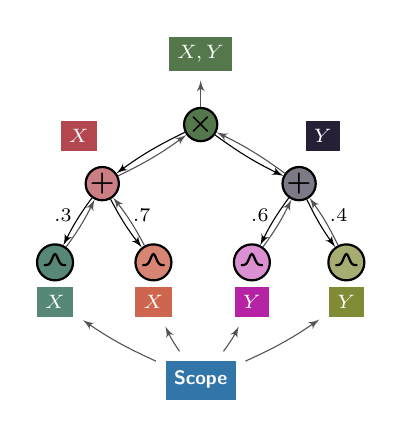
\begin{tikzpicture}
      \newProdNode[fill=boxgreen]{r}{0,0};
      \newSumNode[fill=boxred!70]{p}{$(r) + (-1.25,-0.75)$};
      \newSumNode[fill=boxpurple!60]{q}{$(r) + (1.25,-0.75)$};
      \newGaussNode[fill=boxteal]{x1}{$(p) + (-0.6,-1)$};
      \newGaussNode[fill=boxorange!80]{x2}{$(p) + (0.65,-1)$};
      \newGaussNode[fill=boxpink!50]{y1}{$(q) + (-0.6,-1)$};
      \newGaussNode[fill=boxgoldenrod!70]{y2}{$(q) + (0.6,-1)$};
      \draw[edge] (r) edge[bend right=5] (p);
      \draw[edge] (r) edge[bend right=5] (q);
      \draw[edge] (p) edge[bend right=5] (x1);
      \draw[edge] (p) edge[bend right=5] (x2);
      \draw[edge] (q) edge[bend right=5] (y1);
      \draw[edge] (q) edge[bend right=5] (y2);
      \node at ($(p) + (-0.5,-0.4)$) {\scriptsize$.3$};
      \node at ($(p) + (0.5,-0.4)$) {\scriptsize$.7$};
      \node at ($(q) + (-0.5,-0.4)$) {\scriptsize$.6$};
      \node at ($(q) + (0.5,-0.4)$) {\scriptsize$.4$};
      \node (l1) at ($(x1) + (0,-0.5)$) {\scriptsize\colorbox{boxteal}{\color{white}$X$}};
      \node (l2) at ($(x2) + (0,-0.5)$) {\scriptsize\colorbox{boxorange}{\color{white}$X$}};
      \node (l3) at ($(y1) + (0,-0.5)$) {\scriptsize\colorbox{boxpink}{\color{white}$Y$}};
      \node (l4) at ($(y2) + (0,-0.5)$) {\scriptsize\colorbox{boxgoldenrod}{\color{white}$Y$}};
      \draw[edge,boxdgray] (p) edge[bend left=-5] (r);
      \draw[edge,boxdgray] (q) edge[bend left=-5] (r);
      \draw[edge,boxdgray] (x1) edge[bend left=-5] (p);
      \draw[edge,boxdgray] (x2) edge[bend left=-5] (p);
      \draw[edge,boxdgray] (y1) edge[bend left=-5] (q);
      \draw[edge,boxdgray] (y2) edge[bend left=-5] (q);
      \node at ($(p) + (-0.3,0.6)$) {\scriptsize\colorbox{boxred}{\color{white}$X$}};
      \node at ($(q) + (0.3,0.6)$) {\scriptsize\colorbox{boxpurple}{\color{white}$Y$}};
      \node (sc) at ($(r) + (0,-3.25)$) {\scriptsize\colorbox{boxblue}{\color{white}\strut\textbf{Scope}}};
      \draw[edge,boxdgray] (sc) edge[bend left=5] (l1);
      \draw[edge,boxdgray] (sc) edge[bend left=5] (l2);
      \draw[edge,boxdgray] (sc) edge[bend right=5] (l3);
      \draw[edge,boxdgray] (sc) edge[bend right=5] (l4);
      \node (out) at ($(r) + (0,0.9)$) {\scriptsize\colorbox{boxgreen}{\color{white}$X,Y$}};
      \draw[edge,boxdgray] (r) edge (out);
    \end{tikzpicture}
    }
  \end{vhcenterb}
\end{minipage}
\end{center}

\textcolor{boxdgray}{\cite{darwiche99,darwiche01b}}

% Slide: PC - Structured Decomposability

\newpage

\newtitle{Probabilistic Circuits -- Structured Decomposability}
\vspace*{1cm}

\begin{center}
  \resizebox{!}{0.65\textheight}{
  \centering
  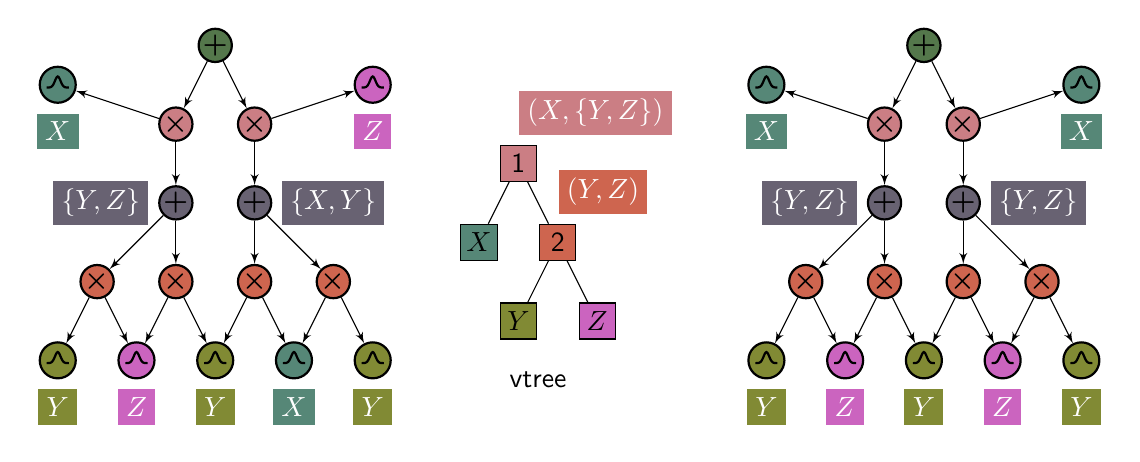
\begin{tikzpicture}
    \newSumNode[fill=boxgreen]{r}{0,0};
    \newProdNode[fill=boxred!70]{p1}{$(r) + (-0.5,-1)$};
    \newProdNode[fill=boxred!70]{p2}{$(r) + (0.5,-1)$};
    \newGaussNode[label=below:{\colorbox{boxteal}{\color{white}$X$}},fill=boxteal]{x1}{$(p1) + (-1.5,0.5)$};
    \newGaussNode[label=below:{\colorbox{boxpink!70}{\color{white}$Z$}},fill=boxpink!70]{z1}{$(p2) + (1.5,0.5)$};
    \newSumNode[label=left:{\colorbox{boxpurple!70}{\color{white}$\{Y,Z\}$}},fill=boxpurple!70]{s1}{$(p1) + (0,-1)$};
    \newSumNode[label=right:{\colorbox{boxpurple!70}{\color{white}$\{X,Y\}$}},fill=boxpurple!70]{s2}{$(p2) + (0,-1)$};
    \newProdNode[fill=boxorange]{q1}{$(s1) + (-1,-1)$};
    \newProdNode[fill=boxorange]{q2}{$(s1) + (0,-1)$};
    \newProdNode[fill=boxorange]{q3}{$(s2) + (0,-1)$};
    \newProdNode[fill=boxorange]{q4}{$(s2) + (1,-1)$};
    \newGaussNode[label=below:{\colorbox{boxgoldenrod}{\color{white}$Y$}},fill=boxgoldenrod]{y1}{$(q1) + (-0.5,-1)$};
    \newGaussNode[label=below:{\colorbox{boxpink!70}{\color{white}$Z$}},fill=boxpink!70]{z2}{$(q2) + (-0.5,-1)$};
    \newGaussNode[label=below:{\colorbox{boxgoldenrod}{\color{white}$Y$}},fill=boxgoldenrod]{y2}{$(q3) + (-0.5,-1)$};
    \newGaussNode[label=below:{\colorbox{boxteal}{\color{white}$X$}},fill=boxteal]{x2}{$(q4) + (-0.5,-1)$};
    \newGaussNode[label=below:{\colorbox{boxgoldenrod}{\color{white}$Y$}},fill=boxgoldenrod]{y3}{$(q4) + (0.5,-1)$};
    \draw[edge] (r) -- (p1);
    \draw[edge] (r) -- (p2);
    \draw[edge] (p1) -- (x1);
    \draw[edge] (p1) -- (s1);
    \draw[edge] (p2) -- (z1);
    \draw[edge] (p2) -- (s2);
    \draw[edge] (s1) -- (q1);
    \draw[edge] (s1) -- (q2);
    \draw[edge] (s2) -- (q3);
    \draw[edge] (s2) -- (q4);
    \draw[edge] (q1) -- (y1);
    \draw[edge] (q2) -- (z2);
    \draw[edge] (q3) -- (y2);
    \draw[edge] (q4) -- (y3);
    \draw[edge] (q1) -- (z2);
    \draw[edge] (q2) -- (y2);
    \draw[edge] (q3) -- (x2);
    \draw[edge] (q4) -- (x2);

    \newVtreeNode[label={[xshift=-0.35cm]above right:{\colorbox{boxred!70}{\color{white}$(X,\{Y,Z\})$}}},fill=boxred!70]{r}{3.85,-1.5}{1};
    \newVtreeNode[label={[xshift=-0.35cm]above right:{\colorbox{boxorange}{\color{white}$(Y,Z)$}}},fill=boxorange]{c}{$(r) + (0.5,-1)$}{2};
    \newVtreeNode[fill=boxteal]{x}{$(r) + (-0.5,-1)$}{$X$};
    \newVtreeNode[fill=boxgoldenrod]{y}{$(c) + (-0.5,-1)$}{$Y$};
    \newVtreeNode[fill=boxpink!70]{z}{$(c) + (0.5,-1)$}{$Z$};
    \node at ($(c) + (-0.25,-1.75)$) {vtree};
    \draw (r) -- (c) -- (y); \draw (c) -- (z); \draw (r) -- (x);

    \newSumNode[fill=boxgreen]{r}{9,0};
    \newProdNode[fill=boxred!70]{p1}{$(r) + (-0.5,-1)$};
    \newProdNode[fill=boxred!70]{p2}{$(r) + (0.5,-1)$};
    \newGaussNode[label=below:{\colorbox{boxteal}{\color{white}$X$}},fill=boxteal]{x1}{$(p1) + (-1.5,0.5)$};
    \newGaussNode[label=below:{\colorbox{boxteal}{\color{white}$X$}},fill=boxteal]{z1}{$(p2) + (1.5,0.5)$};
    \newSumNode[label=left:{\colorbox{boxpurple!70}{\color{white}$\{Y,Z\}$}},fill=boxpurple!70]{s1}{$(p1) + (0,-1)$};
    \newSumNode[label=right:{\colorbox{boxpurple!70}{\color{white}$\{Y,Z\}$}},fill=boxpurple!70]{s2}{$(p2) + (0,-1)$};
    \newProdNode[fill=boxorange]{q1}{$(s1) + (-1,-1)$};
    \newProdNode[fill=boxorange]{q2}{$(s1) + (0,-1)$};
    \newProdNode[fill=boxorange]{q3}{$(s2) + (0,-1)$};
    \newProdNode[fill=boxorange]{q4}{$(s2) + (1,-1)$};
    \newGaussNode[label=below:{\colorbox{boxgoldenrod}{\color{white}$Y$}},fill=boxgoldenrod]{y1}{$(q1) + (-0.5,-1)$};
    \newGaussNode[label=below:{\colorbox{boxpink!70}{\color{white}$Z$}},fill=boxpink!70]{z2}{$(q2) + (-0.5,-1)$};
    \newGaussNode[label=below:{\colorbox{boxgoldenrod}{\color{white}$Y$}},fill=boxgoldenrod]{y2}{$(q3) + (-0.5,-1)$};
    \newGaussNode[label=below:{\colorbox{boxpink!70}{\color{white}$Z$}},fill=boxpink!70]{x2}{$(q4) + (-0.5,-1)$};
    \newGaussNode[label=below:{\colorbox{boxgoldenrod}{\color{white}$Y$}},fill=boxgoldenrod]{y3}{$(q4) + (0.5,-1)$};
    \draw[edge] (r) -- (p1);
    \draw[edge] (r) -- (p2);
    \draw[edge] (p1) -- (x1);
    \draw[edge] (p1) -- (s1);
    \draw[edge] (p2) -- (z1);
    \draw[edge] (p2) -- (s2);
    \draw[edge] (s1) -- (q1);
    \draw[edge] (s1) -- (q2);
    \draw[edge] (s2) -- (q3);
    \draw[edge] (s2) -- (q4);
    \draw[edge] (q1) -- (y1);
    \draw[edge] (q2) -- (z2);
    \draw[edge] (q3) -- (y2);
    \draw[edge] (q4) -- (y3);
    \draw[edge] (q1) -- (z2);
    \draw[edge] (q2) -- (y2);
    \draw[edge] (q3) -- (x2);
    \draw[edge] (q4) -- (x2);
  \end{tikzpicture}
  }
  \vskip 1cm
  \resizebox{\textwidth}{!}{\begin{minipage}{0.675\textwidth}
    \begin{definition}[Structured decomposability]
      \centering
      Every product node follows a vtree decomposition.
    \end{definition}
  \end{minipage}}
\end{center}

\vskip 1cm
\textcolor{boxdgray}{\cite{pipa08}}

% Slide: PC - Logic Circuits

\newpage

\newtitle{Probabilistic Circuits -- Logic Circuits}
\vspace*{0.5cm}

\begin{center}
\begin{minipage}[t][0.8\textheight][t]{0.45\textwidth}
  \begin{vhcenterb}
    \resizebox{!}{0.2\textheight}{
    \begin{tabular}{ccc|c}
      \hline
      $A$ & $B$ & $C$ & $\phi(\set{x})$\\
      \hline
      0 & 0 & 0 & 1 \\
      1 & 0 & 0 & 1 \\
      0 & 1 & 0 & 0 \\
      1 & 1 & 0 & 0 \\
      0 & 0 & 1 & 1 \\
      1 & 0 & 1 & 1 \\
      0 & 1 & 1 & 0 \\
      1 & 1 & 1 & 1 \\
      \hline
    \end{tabular}
    }

    \vskip 0.25cm
    \resizebox{0.8\textwidth}{!}{
    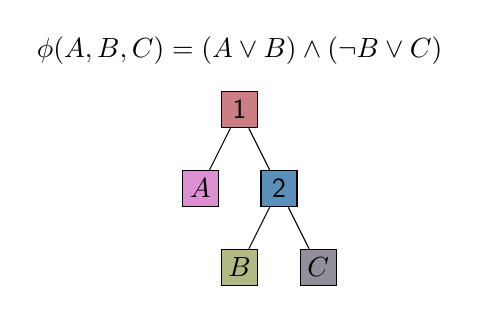
\begin{tikzpicture}
      \node at (0,0) {$\phi(A,B,C)=(A\vee B)\wedge(\neg B\vee C)$};
      \newVtreeNode[fill=boxred!70]{vr}{0,-0.75}{1};
      \newVtreeNode[fill=boxblue!80]{vc}{$(vr) + (0.5,-1)$}{2};
      \newVtreeNode[fill=boxpink!50]{a}{$(vr) + (-0.5,-1)$}{$A$};
      \newVtreeNode[fill=boxgoldenrod!60]{b}{$(vc) + (-0.5,-1)$}{$B$};
      \newVtreeNode[fill=boxpurple!50]{c}{$(vc) + (0.5,-1)$}{$C$};
      \draw (vr) -- (vc) -- (b); \draw (vr) -- (a);
      \draw (vc) -- (c);
    \end{tikzpicture}
    }
  \end{vhcenterb}
\end{minipage}
\begin{minipage}[t][0.8\textheight][t]{0.45\textwidth}
  \begin{vhcenterb}
    \resizebox{0.7\textwidth}{!}{
    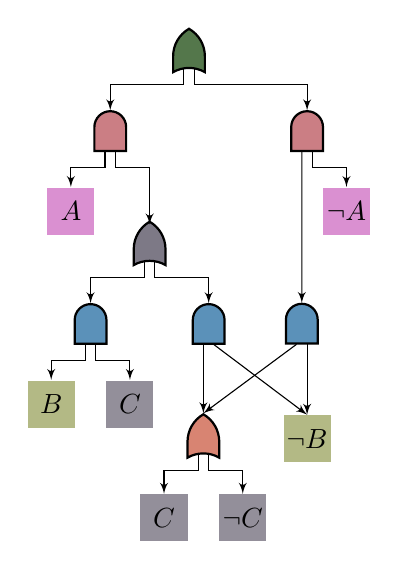
\begin{tikzpicture}
      \newOrNode[inputs=nn,fill=boxgreen]{r}{0,0};
      \newAndNode[inputs=nn,fill=boxred!70]{p1}{$(r) + (-1,-1)$};
      \newAndNode[inputs=nn,fill=boxred!70]{p2}{$(r) + (1.5,-1)$};
      \newLitNode[fill=boxpink!50]{a}{$(p1) + (-0.5,-1)$}{$A$};
      \newOrNode[inputs=nn,fill=boxpurple!60]{s1}{$(p1) + (0.5,-1.45)$};
      \newLitNode[fill=boxpink!50]{na}{$(p2) + (0.5,-1)$}{$\neg A$};
      \newAndNode[inputs=nn,fill=boxblue!80]{q1}{$(s1) + (-0.75,-1)$};
      \newAndNode[inputs=nn,fill=boxblue!80]{q2}{$(s1) + (0.75,-1)$};
      \newAndNode[inputs=nn,fill=boxblue!80]{q3}{$(p2.input 1) + (0,-2.2)$};
      \newLitNode[fill=boxgoldenrod!60]{b}{$(q1) + (-0.5,-1)$}{$B$};
      \newLitNode[fill=boxpurple!50]{c1}{$(q1) + (0.5,-1)$}{$C$};
      \newOrNode[inputs=nn,fill=boxorange!80]{z1}{$(q2.input 1) + (0,-1.2)$};
      \newLitNode[fill=boxgoldenrod!60]{nb}{$(q3.input 2) + (0,-1.2)$}{$\neg B$};
      \newLitNode[fill=boxpurple!50]{c}{$(z1) + (-0.5,-1)$}{$C$};
      \newLitNode[fill=boxpurple!50]{nc}{$(z1) + (0.5,-1)$}{$\neg C$};
      \draw[edge] (r.input 1) -- ++(0,-0.2) -| (p1);
      \draw[edge] (r.input 2) -- ++(0,-0.2) -|  (p2);
      \draw[edge] (s1.input 1) -- ++(0,-0.2) -| (q1);
      \draw[edge] (s1.input 2) -- ++(0,-0.2) -| (q2);
      \draw[edge] (p1.input 1) -- ++(0,-0.2) -| (a.north);
      \draw[edge] (p1.input 2) -- ++(0,-0.2) -| (s1);
      \draw[edge] (p2.input 1) -- (q3);
      \draw[edge] (p2.input 2) -- ++(0,-0.2) -| (na.north);
      \draw[edge] (q1.input 1) -- ++(0,-0.2) -| (b.north);
      \draw[edge] (q1.input 2) -- ++(0,-0.2) -| (c1.north);
      \draw[edge] (q2.input 1) -- (z1.east);
      \draw[edge] (q2.input 2) -- (nb.north);
      \draw[edge] (q3.input 1) -- (z1.east);
      \draw[edge] (q3.input 2) -- (nb.north);
      \draw[edge] (z1.input 1) -- ++(0,-0.2) -| (c);
      \draw[edge] (z1.input 2) -- ++(0,-0.2) -| (nc);
    \end{tikzpicture}
    }
  \end{vhcenterb}
\end{minipage}
\end{center}

\textcolor{boxdgray}{\cite{darwiche11}}

% Slide: PC - Support

\newpage

\newtitle{Probabilistic Circuits -- Support}
\vspace*{0.5cm}

\begin{center}
\begin{minipage}[t][0.8\textheight][t]{0.45\textwidth}
  \begin{vhcenterb}
    \resizebox{!}{0.2\textheight}{
    \begin{tabular}{ccc|cc}
      \hline
      $A$ & $B$ & $C$ & $\phi(\set{x})$ & $p(\set{x})$\\
      \hline
      0 & 0 & 0 & 1 & 0.140\\
      1 & 0 & 0 & 1 & 0.024\\
      0 & 1 & 0 & 0 & \textcolor{gray}{0.000}\\
      1 & 1 & 0 & 0 & \textcolor{gray}{0.000}\\
      0 & 0 & 1 & 1 & 0.560\\
      1 & 0 & 1 & 1 & 0.096\\
      0 & 1 & 1 & 0 & \textcolor{gray}{0.000}\\
      1 & 1 & 1 & 1 & 0.180\\
      \hline
    \end{tabular}
    }

    \vskip 0.25cm
    \resizebox{0.8\textwidth}{!}{
    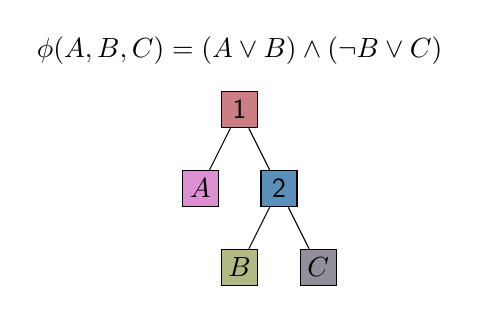
\begin{tikzpicture}
      \node at (0,0) {$\phi(A,B,C)=(A\vee B)\wedge(\neg B\vee C)$};
      \newVtreeNode[fill=boxred!70]{vr}{0,-0.75}{1};
      \newVtreeNode[fill=boxblue!80]{vc}{$(vr) + (0.5,-1)$}{2};
      \newVtreeNode[fill=boxpink!50]{a}{$(vr) + (-0.5,-1)$}{$A$};
      \newVtreeNode[fill=boxgoldenrod!60]{b}{$(vc) + (-0.5,-1)$}{$B$};
      \newVtreeNode[fill=boxpurple!50]{c}{$(vc) + (0.5,-1)$}{$C$};
      \draw (vr) -- (vc) -- (b); \draw (vr) -- (a);
      \draw (vc) -- (c);
    \end{tikzpicture}
    }
  \end{vhcenterb}
\end{minipage}
\begin{minipage}[t][0.8\textheight][t]{0.45\textwidth}
  \begin{vhcenterb}
    \resizebox{0.7\textwidth}{!}{
    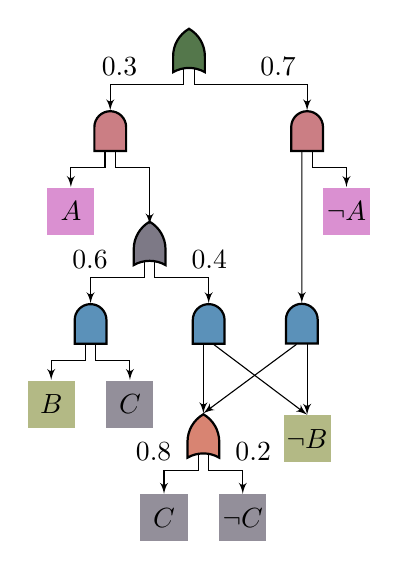
\begin{tikzpicture}
      \newOrNode[inputs=nn,fill=boxgreen]{r}{0,0};
      \newAndNode[inputs=nn,fill=boxred!70]{p1}{$(r) + (-1,-1)$};
      \newAndNode[inputs=nn,fill=boxred!70]{p2}{$(r) + (1.5,-1)$};
      \newLitNode[fill=boxpink!50]{a}{$(p1) + (-0.5,-1)$}{$A$};
      \newOrNode[inputs=nn,fill=boxpurple!60]{s1}{$(p1) + (0.5,-1.45)$};
      \newLitNode[fill=boxpink!50]{na}{$(p2) + (0.5,-1)$}{$\neg A$};
      \newAndNode[inputs=nn,fill=boxblue!80]{q1}{$(s1) + (-0.75,-1)$};
      \newAndNode[inputs=nn,fill=boxblue!80]{q2}{$(s1) + (0.75,-1)$};
      \newAndNode[inputs=nn,fill=boxblue!80]{q3}{$(p2.input 1) + (0,-2.2)$};
      \newLitNode[fill=boxgoldenrod!60]{b}{$(q1) + (-0.5,-1)$}{$B$};
      \newLitNode[fill=boxpurple!50]{c1}{$(q1) + (0.5,-1)$}{$C$};
      \newOrNode[inputs=nn,fill=boxorange!80]{z1}{$(q2.input 1) + (0,-1.2)$};
      \newLitNode[fill=boxgoldenrod!60]{nb}{$(q3.input 2) + (0,-1.2)$}{$\neg B$};
      \newLitNode[fill=boxpurple!50]{c}{$(z1) + (-0.5,-1)$}{$C$};
      \newLitNode[fill=boxpurple!50]{nc}{$(z1) + (0.5,-1)$}{$\neg C$};
      \draw[edge] (r.input 1) -- ++(0,-0.2) -| node[near start,above left] {$0.3$} (p1);
      \draw[edge] (r.input 2) -- ++(0,-0.2) -| node[near start,above right] {$0.7$} (p2);
      \draw[edge] (s1.input 1) -- ++(0,-0.2) -| node[near start,above left] {$0.6$} (q1);
      \draw[edge] (s1.input 2) -- ++(0,-0.2) -| node[near start,above right] {$0.4$} (q2);
      \draw[edge] (p1.input 1) -- ++(0,-0.2) -| (a.north);
      \draw[edge] (p1.input 2) -- ++(0,-0.2) -| (s1);
      \draw[edge] (p2.input 1) -- (q3);
      \draw[edge] (p2.input 2) -- ++(0,-0.2) -| (na.north);
      \draw[edge] (q1.input 1) -- ++(0,-0.2) -| (b.north);
      \draw[edge] (q1.input 2) -- ++(0,-0.2) -| (c1.north);
      \draw[edge] (q2.input 1) -- (z1.east);
      \draw[edge] (q2.input 2) -- (nb.north);
      \draw[edge] (q3.input 1) -- (z1.east);
      \draw[edge] (q3.input 2) -- (nb.north);
      \draw[edge] (z1.input 1) -- ++(0,-0.2) -| node[near start,above left] {$0.8$} (c);
      \draw[edge] (z1.input 2) -- ++(0,-0.2) -| node[near start,above right] {$0.2$} (nc);
    \end{tikzpicture}
    }
  \end{vhcenterb}
\end{minipage}
\end{center}

\textcolor{boxdgray}{\cite{kisa14}}

% Slide: PC - Tractability

\newpage

\newtitle{Probabilistic Circuits -- Tractability}

\begin{vhcenterb}
  \resizebox{0.75\textwidth}{!}{
  \begin{tabular}{lcccc}
    \hline
    \textbf{Query} & \textbf{+Sm?} & \textbf{+Dec?} & \textbf{+Det?} & \textbf{+Str Dec?} \\
    \hline
    Evidence & \cmark & \cmark & \cmark & \cmark\\
    Marginals & \xmark & \cmark & \cmark & \cmark\\
    Conditionals & \xmark & \cmark & \cmark & \cmark\\
    MPE & \xmark & \xmark & \cmark & \cmark\\
    Shannon Entropy & \xmark & \xmark & \cmark & \cmark\\
    Rényi Entropy & \xmark & \xmark & \cmark & \cmark\\
    Cross Entropy & \xmark & \xmark & \xmark & \cmark\\
    Kullback-Leibler Div& \xmark & \xmark & \xmark & \cmark\\
    Rényi's Alpha Div & \xmark & \xmark & \xmark & \cmark\\
    Cauchy-Schwarz Div & \xmark & \xmark & \xmark & \cmark\\
    Logical Events & \xmark & \xmark & \xmark & \cmark\\
    Mutual Information & \xmark & \xmark & \xmark & \cmark\\
    \hline
  \end{tabular}
  }
\end{vhcenterb}

\textcolor{boxdgray}{\cite{vergari21,poon11,peharz16}}

% Slide: PC - Where are we now?

\newpage

\newtitle{Learning Probabilistic Circuits -- Where are we right now?}

\begin{vhcenterb}
  \newcommand{\divclass}{\textproc{DIV}}
  \newcommand{\incrclass}{\textproc{INCR}}
  \newcommand{\randclass}{\textproc{RAND}}
  \resizebox{0.95\textwidth}{!}{
  \begin{tabular}{c|clcc|cccc|ccc|c}
    \hline
    \textbf{Name} & \textbf{Class} & \multicolumn{1}{c}{\textbf{Time Complexity}} & \textbf{\# hyperparams}
    & \textbf{Accepts logic?} & \textbf{Sm?} & \textbf{Dec?} & \textbf{Det?} & \textbf{Str Dec?} &
    \textbf{$\mathbf{\{0,1\}}$?} & $\mathbb{N}$\textbf{?} & $\mathbb{R}$\textbf{?} & \textbf{Reference}\\
    \hline
    \textproc{LearnSPN} & \divclass{} & $
    \begin{cases}
      \bigo\left(nkmc\right) & \text{, if sum}\\
      \bigo\left(nm^3\right) & \text{, if product}
    \end{cases}
    $ & $\geq 2$ & \xmark & \cmark & \cmark & \xmark & \xmark & \cmark & \cmark & \cmark & \cite{gens13}\\
    \textproc{ID-SPN} & \divclass{} & $
    \begin{cases}
      \bigo\left(nkmc\right) & \text{, if sum}\\
      \bigo\left(nm^3\right) & \text{, if product}\\
      \bigo\left(ic(rn+m)\right)  & \text{, if input}
    \end{cases}
    $ & $\geq 2+3$ & \xmark & \cmark & \cmark & \xmark & \xmark & \cmark & \cmark & \xmark & \cite{rooshenas14}\\
    \textproc{Prometheus} & \divclass{} & $
    \begin{cases}
      \bigo\left(nkmc\right) & \text{, if sum}\\
      \bigo\left(m(\log m)^2\right) & \text{, if product}
    \end{cases}
    $ & $\geq 1$ & \xmark & \cmark & \cmark & \xmark & \xmark & \cmark & \cmark & \cmark & \cite{jaini18a}\\
    \hline
    \textproc{LearnPSDD} & \incrclass{} & $
    \begin{cases}
      \bigo\left(m^2\right) & \text{, top-down vtree}\\
      \bigo\left(m^4\right) & \text{, bottom-up vtree}\\
      \bigo\left(i|\mathcal{C}|^2\right) & \text{, circuit structure}
    \end{cases}
    $ & $1$ & \cmark & \cmark & \cmark & \cmark & \cmark & \cmark & \xmark & \xmark & \cite{liang17}\\
    \textproc{Strudel} & \incrclass{} & $
    \begin{cases}
      \bigo\left(m^2 n\right) & \text{, CLT + vtree}\\
      \bigo\left(i\left(|\mathcal{C}|n+m^2\right)\right) & \text{, circuit structure}
    \end{cases}
    $ & $1$ & \cmark & \cmark & \cmark & \cmark & \cmark & \cmark & \xmark & \xmark & \cite{dang20}\\
    \hline
    & & & & & & & & & & & & \\
    \textproc{RAT-SPN} & \randclass{} & $\phantom{\{}\bigo\left(rd(s+l)\right)$ & $4$ & \xmark & \cmark & \cmark
                       & \xmark & \xmark & \cmark & \cmark & \cmark & \cite{peharz20a}\\
    & & & & & & & & & & & & \\
    \textproc{XPC} & \randclass{} & $\phantom{\{}\bigo\left(i(t+kn)+ikm^2n\right)$ & $3$ & \xmark &\cmark & \cmark
                   & \cmark & \cmark & \cmark & \xmark & \xmark & \cite{dimauro21}\\
    & & & & & & & & & & & & \\
    \noalign{\global\arrayrulewidth=2pt}
    \arrayrulecolor{boxblue}
    \hline
    \noalign{\global\arrayrulewidth=0.4pt}
    \textproc{SamplePSDD} & \randclass{} & $
    \begin{cases}
      \bigo\left(m\right) & \text{, random vtree}\\
      \bigo\left(kc\log c+\log_2^2 k\right) & \text{, per call}
    \end{cases}
    $ & $1$ & \cmark & \cmark & \cmark & \cmark & \cmark & \cmark & \xmark & \xmark & \cite{geh21a}\\
    \textproc{LearnRP} & \randclass{} & $
    \begin{cases}
      \bigo\left(m^2\right) & \text{, top-down vtree}\\
      \bigo\left(m^4\right) & \text{, bottom-up vtree}\\
      \bigo\left(knm\right) & \text{, per call}
    \end{cases}
    $ & $0$ & \xmark & \cmark & \cmark & \xmark & \cmark & \cmark & \cmark & \cmark & To appear \\
    \noalign{\global\arrayrulewidth=2pt}
    \arrayrulecolor{boxblue}
    \hline
  \end{tabular}
  }
\end{vhcenterb}

% Slide: SamplePSDD

\newpage



\nobibliography{refs.bib}

\end{document}
